\documentclass[8pt, oneside]{beamer}   	% use "amsart" instead of "article" for AMSLaTeX format
\usepackage{geometry}                		% See geometry.pdf to learn the layout options. There are lots.
%\geometry{letterpaper}                   		% ... or a4paper or a5paper or ... 
%\geometry{landscape}                		% Activate for rotated page geometry
%\usepackage[parfill]{parskip}    		% Activate to begin paragraphs with an empty line rather than an indent
\usepackage{graphicx}				% Use pdf, png, jpg, or eps§ with pdflatex; use eps in DVI mode
								% TeX will automatically convert eps --> pdf in pdflatex		
\usepackage{amssymb}
\usepackage{amsmath}
\usepackage{textpos} % package for the positioning
\usepackage{eso-pic}


\usepackage {tikz}
\usetikzlibrary {positioning}
\definecolor {processblue}{cmyk}{0.96,0,0,0}

%SetFonts

%SetFonts
\newcommand{\supp}{\operatorname{supp}}
\newcommand{\dist}{\operatorname{dist}}
\newcommand{\divr}{\operatorname{div}}
\newcommand{\tdiv}{\operatorname{div}}
\newcommand{\ess}{\operatorname{ess}}
\newcommand{\rotore}{\operatorname{rot}}
\newcommand{\curl}{\operatorname{\textbf{curl}}}
\newcommand{\bcurl}{\operatorname{\textbf{curl}}}
\newcommand{\tr}{\operatorname{tr}}
\newcommand{\bA}{\textbf{A}}
\newcommand{\ba}{\textbf{a}}
\newcommand{\bb}{\textbf{b}}
\newcommand{\bB}{\textbf{B}}
\newcommand{\bc}{\textbf{c}}
\newcommand{\bC}{\textbf{C}}
\newcommand{\bd}{\textbf{d}}
\newcommand{\bD}{\textbf{D}}
\newcommand{\be}{\textbf{e}}
\newcommand{\bE}{\textbf{E}}
\newcommand{\bff}{\textbf{f}}
\newcommand{\bF}{\textbf{F}}
\newcommand{\bg}{\textbf{g}}
\newcommand{\bG}{\textbf{G}}
\newcommand{\bi}{\textbf{i}}
\newcommand{\bI}{\textbf{I}}
\newcommand{\bj}{\textbf{j}}
\newcommand{\bJ}{\textbf{J}}
\newcommand{\bh}{\textbf{h}}
\newcommand{\bH}{\textbf{H}}
\newcommand{\bk}{\textbf{k}}
\newcommand{\bK}{\textbf{K}}
\newcommand{\bl}{\textbf{l}}
\newcommand{\bL}{\textbf{L}}
\newcommand{\bm}{\textbf{m}}
\newcommand{\bM}{\textbf{M}}
\newcommand{\bn}{\textbf{n}}
\newcommand{\bN}{\textbf{N}}
\newcommand{\bp}{\textbf{p}}
\newcommand{\bP}{\textbf{P}}
\newcommand{\bo}{\textbf{o}}
\newcommand{\bq}{\textbf{q}}
\newcommand{\bQ}{\textbf{Q}}
\newcommand{\br}{\textbf{r}}
\newcommand{\bR}{\textbf{R}}
\newcommand{\bs}{\textbf{s}}
\newcommand{\bS}{\textbf{S}}
\newcommand{\btau}{\boldsymbol{\tau}}
\newcommand{\bt}{\textbf{t}}
\newcommand{\bv}{\textbf{v}}
\newcommand{\bV}{\textbf{V}}
\newcommand{\bw}{\textbf{w}}
\newcommand{\bW}{\textbf{W}}
\newcommand{\bu}{\textbf{u}}
\newcommand{\bU}{\textbf{U}}
\newcommand{\by}{\textbf{y}}
\newcommand{\bY}{\textbf{Y}}
\newcommand{\bbx}{\textbf{x}}
\newcommand{\bX}{\textbf{X}}
\newcommand{\blambda}{\boldsymbol{\lambda}}
\newcommand{\beps}{\boldsymbol{\varepsilon}}
\newcommand{\bphi}{\boldsymbol{\phi}}
\newcommand{\bPhi}{\boldsymbol{\Phi}}
\newcommand{\bpsi}{\boldsymbol{\psi}}
\newcommand{\bomega}{\boldsymbol{\omega}}
\newcommand{\bsigma}{\boldsymbol{\sigma}}
\newcommand{\bSigma}{\boldsymbol{\Sigma}}
\newcommand{\bxi}{\boldsymbol{\xi}}
\newcommand{\aaa}{\`a}
\newcommand{\eee}{\`e}
\newcommand{\iii}{\`i}
\newcommand{\ooo}{\`o}
\newcommand{\uuu}{\`u}
\newcommand{\aaaa}{\'a}
\newcommand{\eeee}{\'e}
\newcommand{\iiii}{\'i}
\newcommand{\oooo}{\'o}
\newcommand{\uuuu}{\'u}
\newcommand{\AAA}{\`A}
\newcommand{\EEE}{\`E}
\newcommand{\III}{\`I}
\newcommand{\OOO}{\`O}
\newcommand{\UUU}{\`U}
\newcommand{\AAAA}{\'A}
\newcommand{\EEEE}{\'E}
\newcommand{\IIII}{\'I}
\newcommand{\OOOO}{\'O}
\newcommand{\UUUU}{\'U}
\newcommand{\ND}{\mathcal{ND}}
\newcommand{\RT}{\mathcal{RT}}

%%% norm and abs
\newcommand\norm[1]{\left\lVert#1\right\rVert}
\newcommand\abs[1]{\left\vert#1\right\vert}


\usepackage[utf8]{inputenc}
\usetheme{PaloAlto}
\definecolor{Colorrr}{rgb}{1, 0.88, 0.5}
\usecolortheme[named=Colorrr]{structure}
%\logo{
\includegraphics[width=1.16cm,height=1.16cm]{img/logo_ics2}\vspace{1pt}\hspace{-10000pt}}

\newcommand\AtPagemyUpperLeft[1]{\AtPageLowerLeft{%
\put(\LenToUnit{0.81\paperwidth},\LenToUnit{0.881\paperheight}){#1}}}
\AddToShipoutPictureFG{
  \AtPagemyUpperLeft{{
\includegraphics[width=2.5cm,keepaspectratio]{img/logo_ics}}}
}%



\setbeamercolor{frametitle}{fg=black}

\usepackage{color}
% Colors
%------------------------------------------------------------------------------------------------------------------------------------------
\definecolor{bgblue}{rgb}{0.04,0.39,0.53}
\definecolor{dkgreen}{cmyk}{1,0.58,1,0.33}
\definecolor{mygreen}{rgb}{0,0.6,0}
\definecolor{bgorange}{cmyk}{0,0.1,0.7,0}
\definecolor{orange}{cmyk}{0,0.9,0.9,0}
\definecolor{navyblue}{cmyk}{1,0.7,0.36,0.4}
\definecolor{brown}{cmyk}{0.62,0.79,0.93,0.22}
\definecolor{tan}{cmyk}{0.14,0.21,0.47,0}
\definecolor{dkgrey}{cmyk}{0.72,0.7,0.75,0.15}

\newcommand{\colr}{\color{red}}
\newcommand{\colb}{\color{blue}}
\newcommand{\colg}{\color{mygreen}}
\newcommand{\colo}{\color{orange}}
\newcommand{\colw}{\color{white}}
\newcommand{\colt}{\color{tan}}
\newcommand{\coln}{\color{brown}}
\newcommand{\colk}{\color{black}}
\newcommand{\colc}{\color{cyan}}
\newcommand{\colm}{\color{magenta}}
\newcommand{\coly}{\color{yellow}}


\newcommand{\titlecolor}[1]{\frametitle{\textcolor{dkgrey}{ \textbf{#1}}}}
%------------------------------------------------------------------------------------------------------------------------------------------




%\addtobeamertemplate{frametitle}{}{%
%\begin{textblock*}{100mm}(\textwidth,-0.84cm)
%
\includegraphics[height=1.5cm,width=1.5cm,keepaspectratio]{img/logo}
%\end{textblock*}}
 
%------------------------------------------------------------------------------------------------------------------------------------------

% titlepage definitions
%------------------------------------------------------------------------------------------------------------------------------------------

\title{ \textcolor{dkgrey}{  \textbf{Monotone multilevel for FOSLS linear elastic contact} }}
\author{\textcolor{dkgrey}{G. Rovi, B. Kober, G. Starke, R. Krause}}
\institute{Universit\"at Duisburg\,-\,Essen, Germany \\ Universit\aaa~della Svizzera italiana, Switzerland}





\begin{document}
 \begin{frame}
\titlepage
\begin{figure}[htbp!]
	
\includegraphics[scale=0.7]{img/logo_ics}
	\quad
		
\includegraphics[scale=0.3]{img/essenlogo}
\end{figure}
\end{frame}








 



%%%%%%%%%%%%%%%%%%%%%%%%%%%%%%%%%%%%%%%%%%
%%%%%%%%%%%                   SLIDE 1                %%%%%%%%%%%%%%%
%%%%%%%%%%%%%%%%%%%%%%%%%%%%%%%%%%%%%%%%%%
\begin{frame}
\titlecolor{Examples of contact problems}
\begin{figure}[htbp!]
	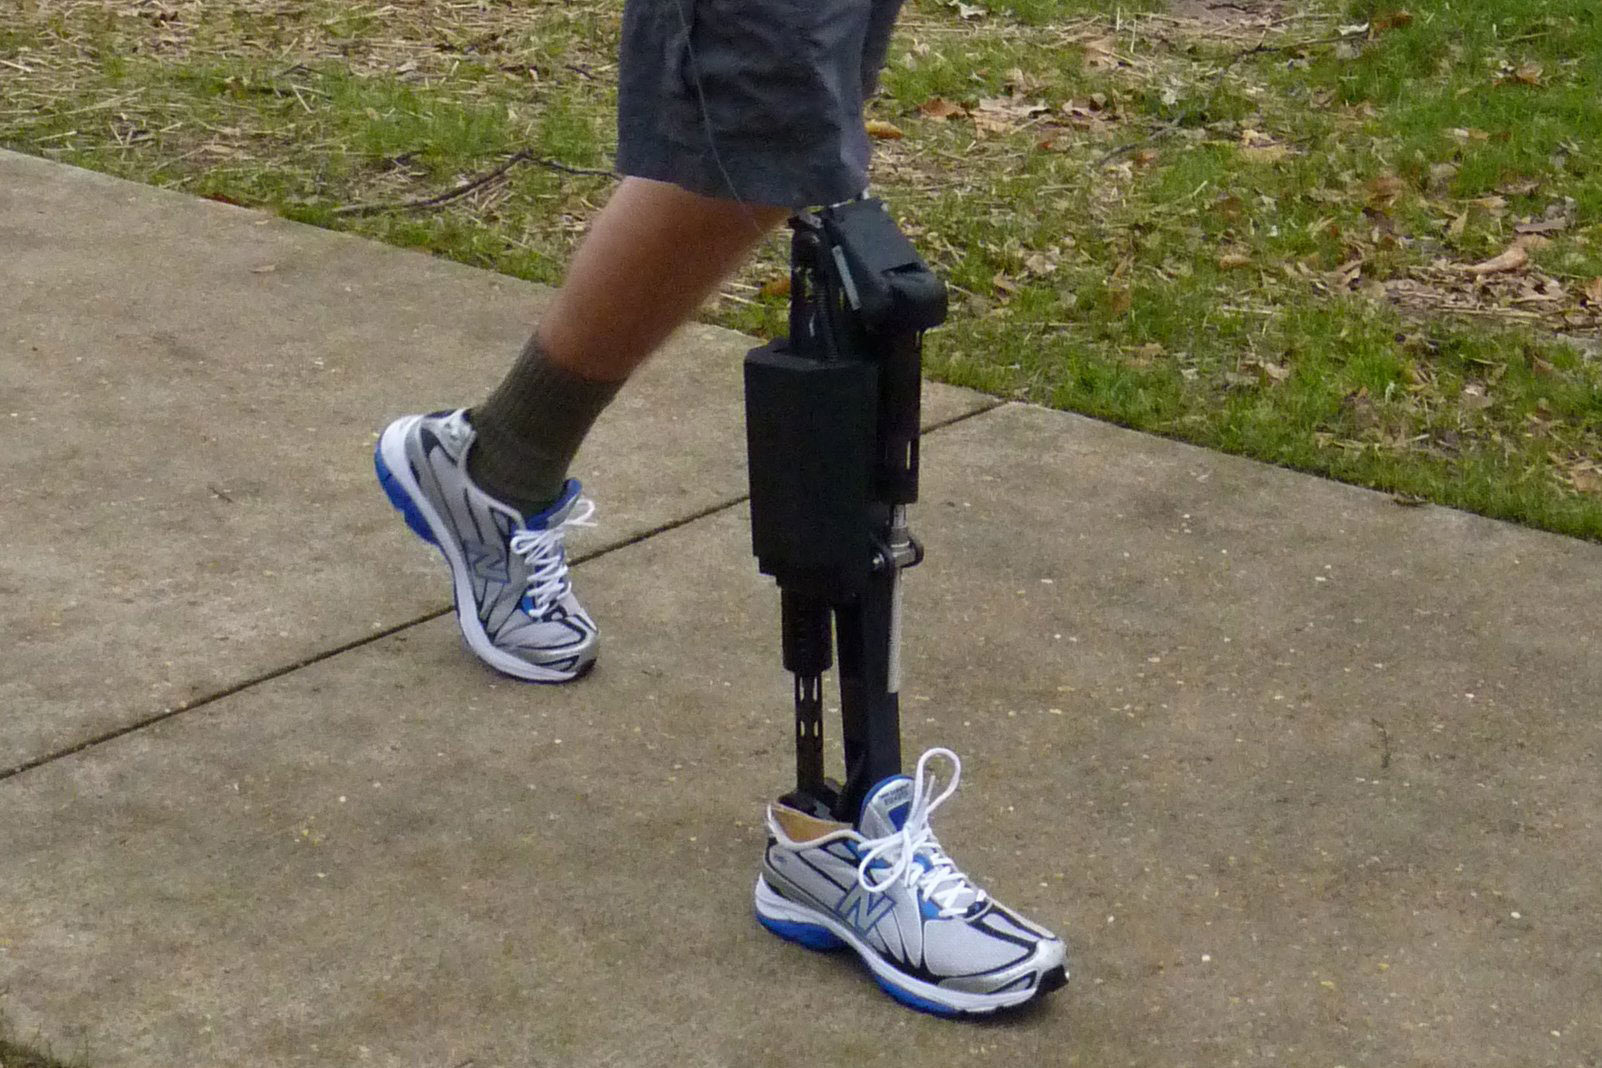
\includegraphics[width=0.35\textwidth]{img/walking}
		\label{abb_arc}\qquad 
			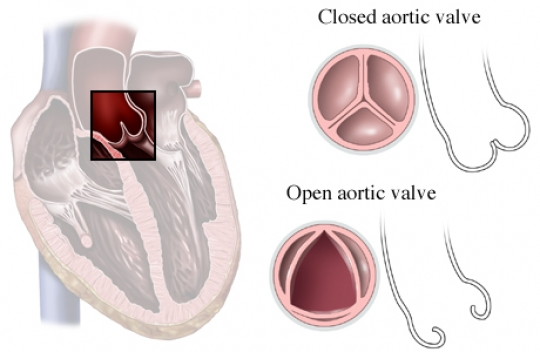
\includegraphics[width=0.35\textwidth]{img/aorticvalve}
		\label{abb_arc}
\end{figure}
\begin{figure}[htbp!]
		\centering
	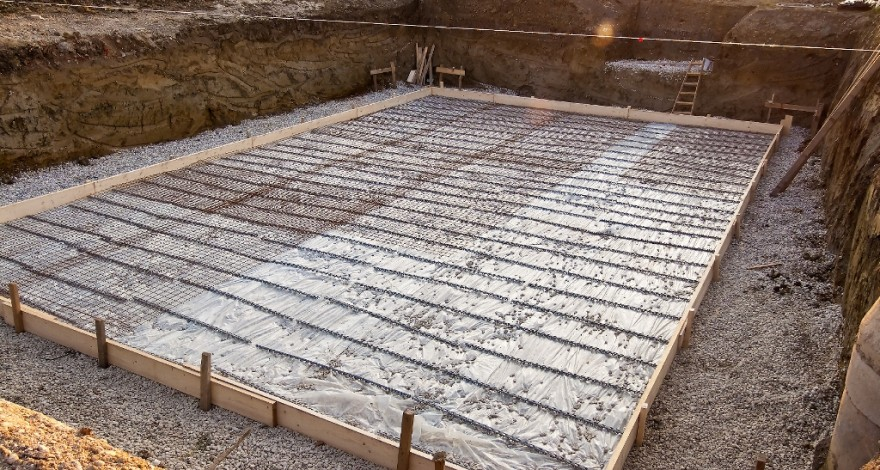
\includegraphics[width=0.4\textwidth]{img/foundation}
		\label{abb_arc}
\end{figure}
\begin{itemize}
\item Contact problems with incompressible materials. 
\item Quantities of interest: the forces generated by the contact.
\end{itemize}
\end{frame}


%%%%%%%%%%%%%%%%%%%%%%%%%%%%%%%%%%%%%%%%%%
%%%%%%%%%%%                   SLIDE 2                %%%%%%%%%%%%%%%
%%%%%%%%%%%%%%%%%%%%%%%%%%%%%%%%%%%%%%%%%%
\begin{frame}
\titlecolor{Signorini's problem: strong formulation}
%\begin{flushleft}
\begin{itemize}
\item  \textbf{Linear Elasticity:}
\scriptsize
\begin{align*}
\colk
\footnotesize
\begin{cases}
\text{div} \bsigma + \bff=0 & \Omega  \qquad \colk{\text{momentum balance equation}}\\
\mathcal{A} \bsigma - \boldsymbol{\varepsilon}(\bu)=0 &\Omega \qquad \colk{\text{constitutive law}}\\
\colb \bu = \bu_D & \colb \Gamma_D\quad \:\:\: \colk{{\text{Dirichlet BC}}}\\
\colg \bsigma  \bn = \bt_N & \colg \Gamma_N\quad  \:\:\:\colk{{\text{Neumann BC}}}\\
\end{cases} \\
\end{align*}
\normalsize
\item { \textbf{Contact Constraints:} }\\
\scriptsize
\colk
$ \partial \Omega=\Gamma_C \cup  \Gamma_D \cup  \Gamma_N$, $\Gamma_i \cap  \Gamma_j =\emptyset$ for $i,j=D,N,C, i \neq j$
\end{itemize}
\begin{align*}\colo
\footnotesize
\begin{cases}
\bu \cdot \bn - g  \leq 0 \quad & \Gamma_C  \:\:  \colk{\text{impenetrability}}\\
(\bsigma \bn) \cdot \bn \leq 0 \quad & \Gamma_C  \:\:  \colk{\text{direction of the surface pressure}}\\
 \left(\bu \cdot \bn -g \right) \left( (\bsigma \bn) \cdot \bn \right) =0 &\Gamma_C  \:\:  \colk{\text{complementarity condition}}\\
  \bt_j^T(\bsigma \bn_j) =0  \quad & \Gamma_C  \:\: \colk{\text{frictionless condition}}
\end{cases}
\end{align*}
%\end{flushleft}
\begin{figure}[htbp!]
		\centering
	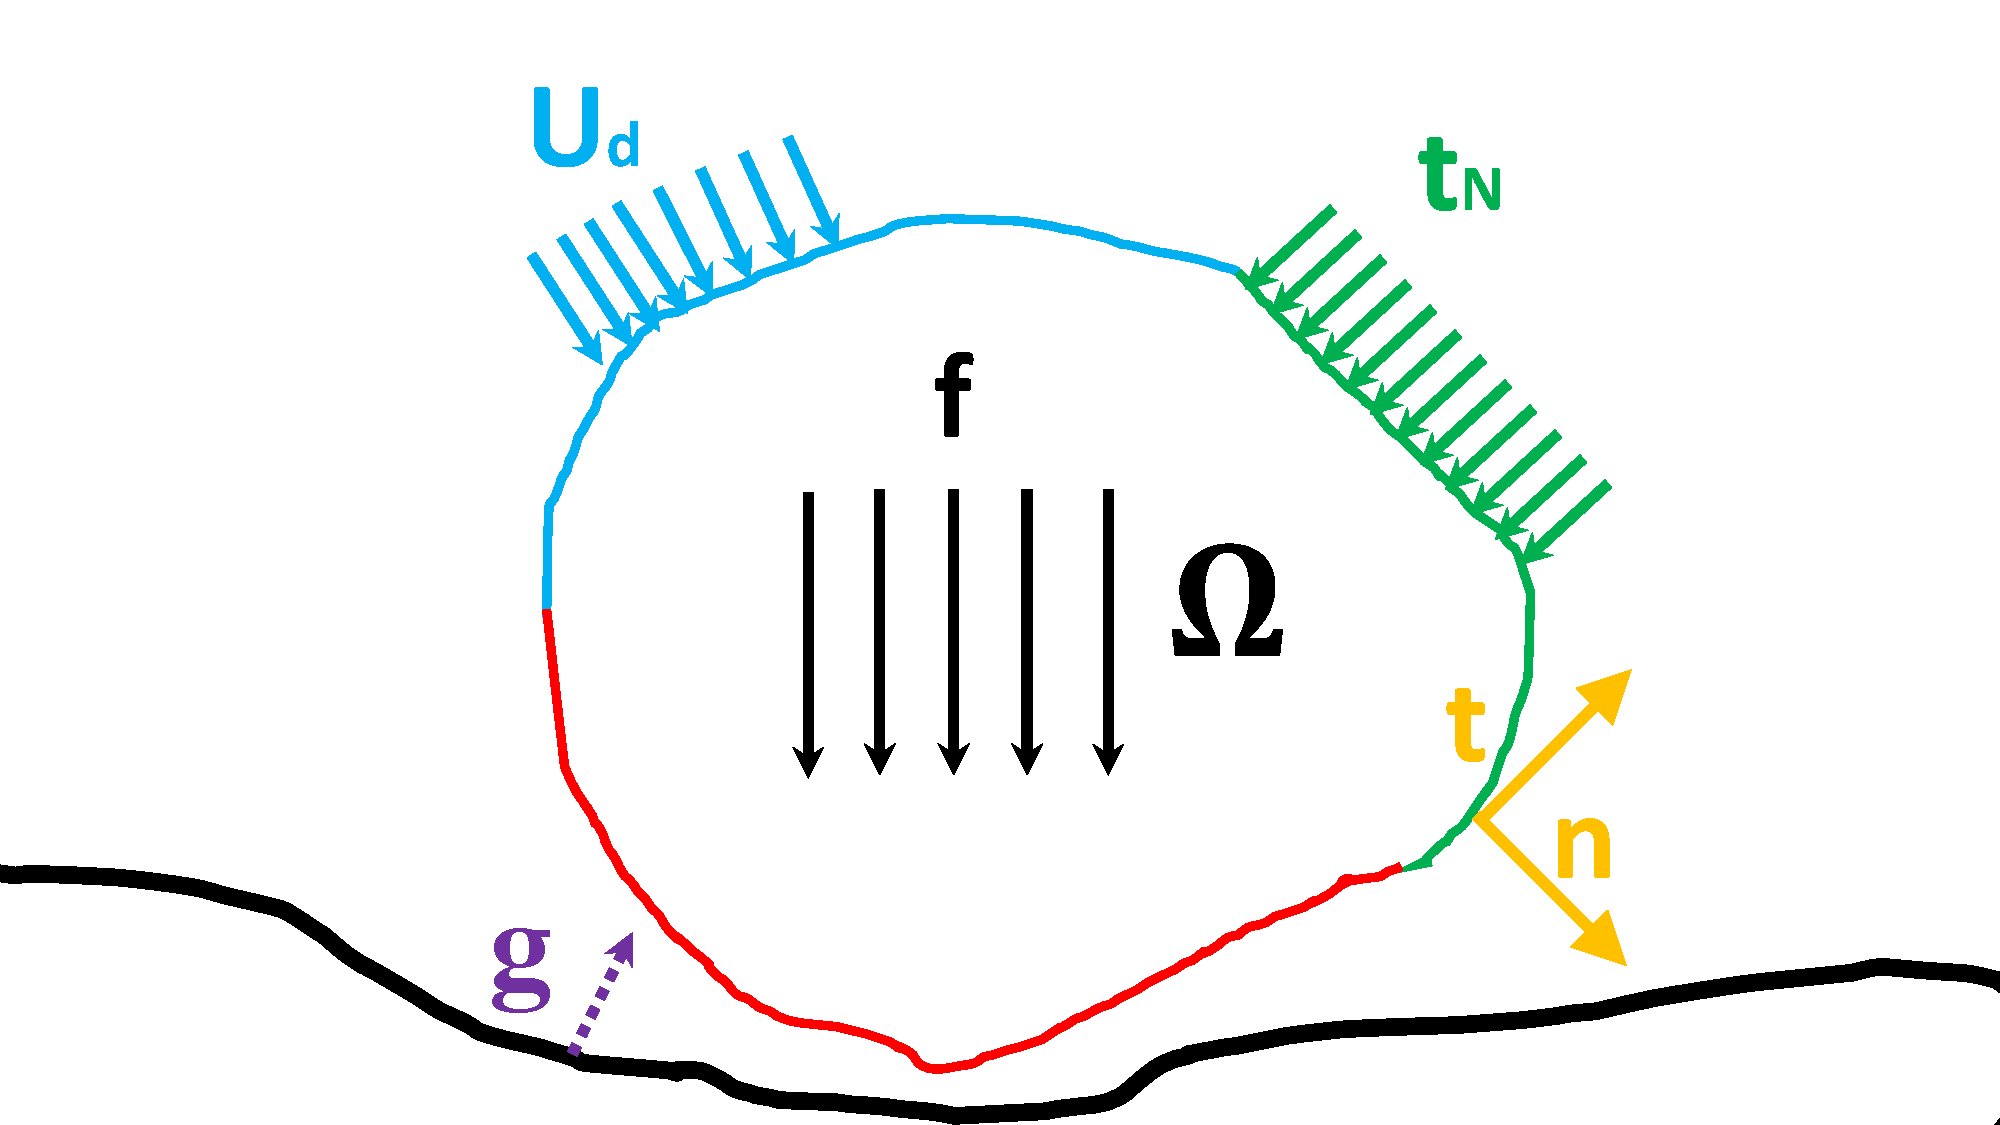
\includegraphics[width=0.35\textwidth]{img/contactproblem.pdf}\qquad
	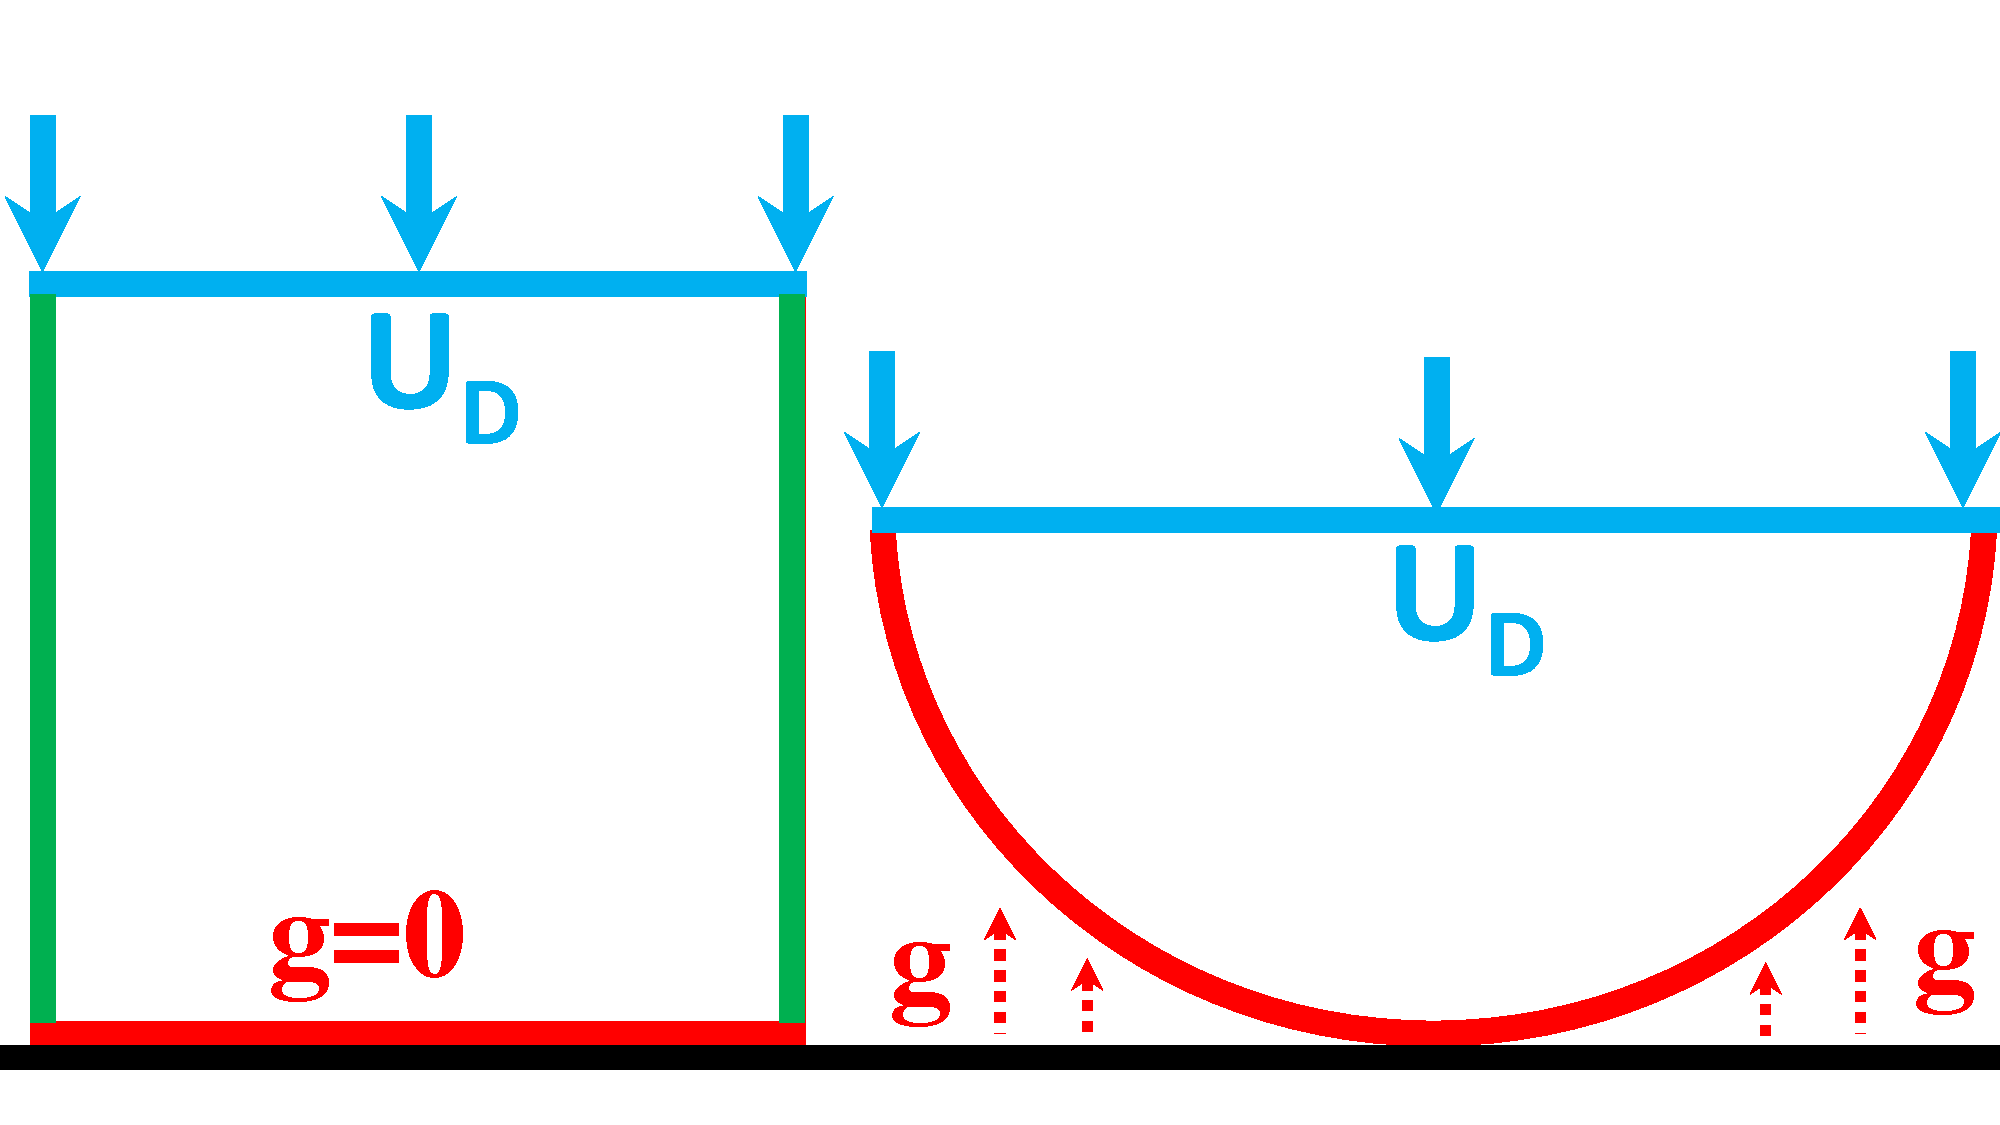
\includegraphics[width=0.35\textwidth]{img/squarecircle.pdf}
		\label{abb_arc}
\end{figure}
%\tiny{Rolf Krause. A nonsmooth multiscale method for solving frictional two-body contact problems in 2d and 3d with multigrid efficiency. SIAM Journal on Scientific Computing, 31(2):1399-1423, 2009.}
\end{frame}


%%%%%%%%%%%%%%%%%%%%%%%%%%%%%%%%%%%%%%%%%%
%%%%%%%%%%%                   SLIDE 3                %%%%%%%%%%%%%%%
%%%%%%%%%%%%%%%%%%%%%%%%%%%%%%%%%%%%%%%%%%

\begin{frame}
\titlecolor{The Least-Squares Formulation}
\begin{itemize}
\item \textbf{First Order System Least-Squares (FOSLS) Functional}
\small
\begin{align*}
& C_1, \:C_2, \: C_3>0 \\
&\mathcal{J}(\bu,\bsigma)=C_{1} \norm{\text{div} \bsigma+\bff}_{L^2(\Omega)^d}^2+C_{2} \norm{\mathcal{A}\bsigma -\boldsymbol{\varepsilon}(\bu)}_{L^2(\Omega)^d}^2   +C_{3} \langle \bu \cdot \bn -g, (\bsigma \bn) \cdot \bn \rangle_{\Gamma_c}
\end{align*} 
${}$\\
\item  
\normalsize
\textbf{Convex Set} $K$
\small
\begin{align*}
& K=\{  \left(\bu,  \bsigma \right)  \in  \left[H_{\Gamma_{d}}^1(\Omega) \right]^d \times \left[ H_{\text{div},\Gamma_N}(\Omega) \right]^d    : \: 
 \bu \cdot \bn - g  \leq 0, \:  (\bsigma \bn) \cdot \bn \leq 0,  \: \bt_j^T(\bsigma \bn_j) =0 \quad  \Gamma_C
 \}
\end{align*}
${}$\\
\item \normalsize 
Find $(\bu,\bsigma) \in K$, such that:
\small
\begin{align*}
\bullet \textbf{Minimization problem:} \qquad  &{ \mathcal{J}(\bu,\bsigma) \leq \mathcal{J}(\bv,\btau ) \qquad \forall (\bv,\btau) \in K}\\\\
&\iff\\\\
\bullet \textbf{Variational Inequality:}\qquad &{
\begin{cases}
&
\left\langle \dfrac{\partial \mathcal{J}(\bu,\bsigma;\bff,g)}{\partial \bu }, \bv-\bu \right\rangle 
\geq 0 \\\\
&
\left\langle \dfrac{\partial \mathcal{J}(\bu,\bsigma;\bff,g)}{\partial \bsigma }, \btau-\bsigma \right\rangle 
\geq 0 
\end{cases}
\qquad \qquad
\forall (\bv, \btau) \in K}
\end{align*}
\end{itemize}
\normalsize
${}$\\
${}$\\${}$\\
\tiny{Rolf Krause, Benjamin M\"{u}ller, and Gerhard Starke. An adaptive least-squares mixed finite element method for the Signorini problem. Numerical Methods for Partial Differential Equations, 33(1):276-289, 2017.}


\end{frame}



%%%%%%%%%%%%%%%%%%%%%%%%%%%%%%%%%%%%%%%%%%
%%%%%%%%%%%                   SLIDE 4                %%%%%%%%%%%%%%%
%%%%%%%%%%%%%%%%%%%%%%%%%%%%%%%%%%%%%%%%%%


\begin{frame}
\titlecolor{Disadvantages and Advantages of the LS formulation}
 \textbf{Advantages of the Least-Squares Approach}
\begin{itemize} 
\item Direct access to stress $\bsigma$ (friction, plasticity...)
\item Dealing with incompressible materials ($\lambda \to \infty$)
\item FOSLS functional as an a posteriori error estimator
\item Flexible choice of finite element spaces (low order: $\bu_h \in P^1$, $\bsigma_h \in \RT_0$)
\item Symmetric positive definite system
\end{itemize}
${}$\\
 \textbf{Disadvantages of the Least-Squares Approach}
\begin{itemize} 
\item The functional is fictitious, not physical
\item The asymmetry of the stress tensor
\item Find proper weights $C_1$, $C_2$, $C_3$
\item Large condition number: need for a \textbf{multilevel method}
\end{itemize}
${}$\\
${}$\\
${}$\\
\tiny{Attia, Frank S., Zhiqiang Cai, and Gerhard Starke. "First-order system least squares for the Signorini contact problem in linear elasticity". SIAM Journal on Numerical Analysis 47.4 (2009): 3027-3043.}\\
\end{frame}






%%%%%%%%%%%%%%%%%%%%%%%%%%%%%%%%%%%%%%%%%%
%%%%%%%%%%%                   SLIDE 5                %%%%%%%%%%%%%%%
%%%%%%%%%%%%%%%%%%%%%%%%%%%%%%%%%%%%%%%%%%
\begin{frame}
\titlecolor{$H^1$ and $H_{\text{div}}$ Multilevel}
\footnotesize
 $\bullet$ A proper smoother must smooth error components related to the large eigenvalues of the system operator; 
 \begin{figure}[htbp!]
	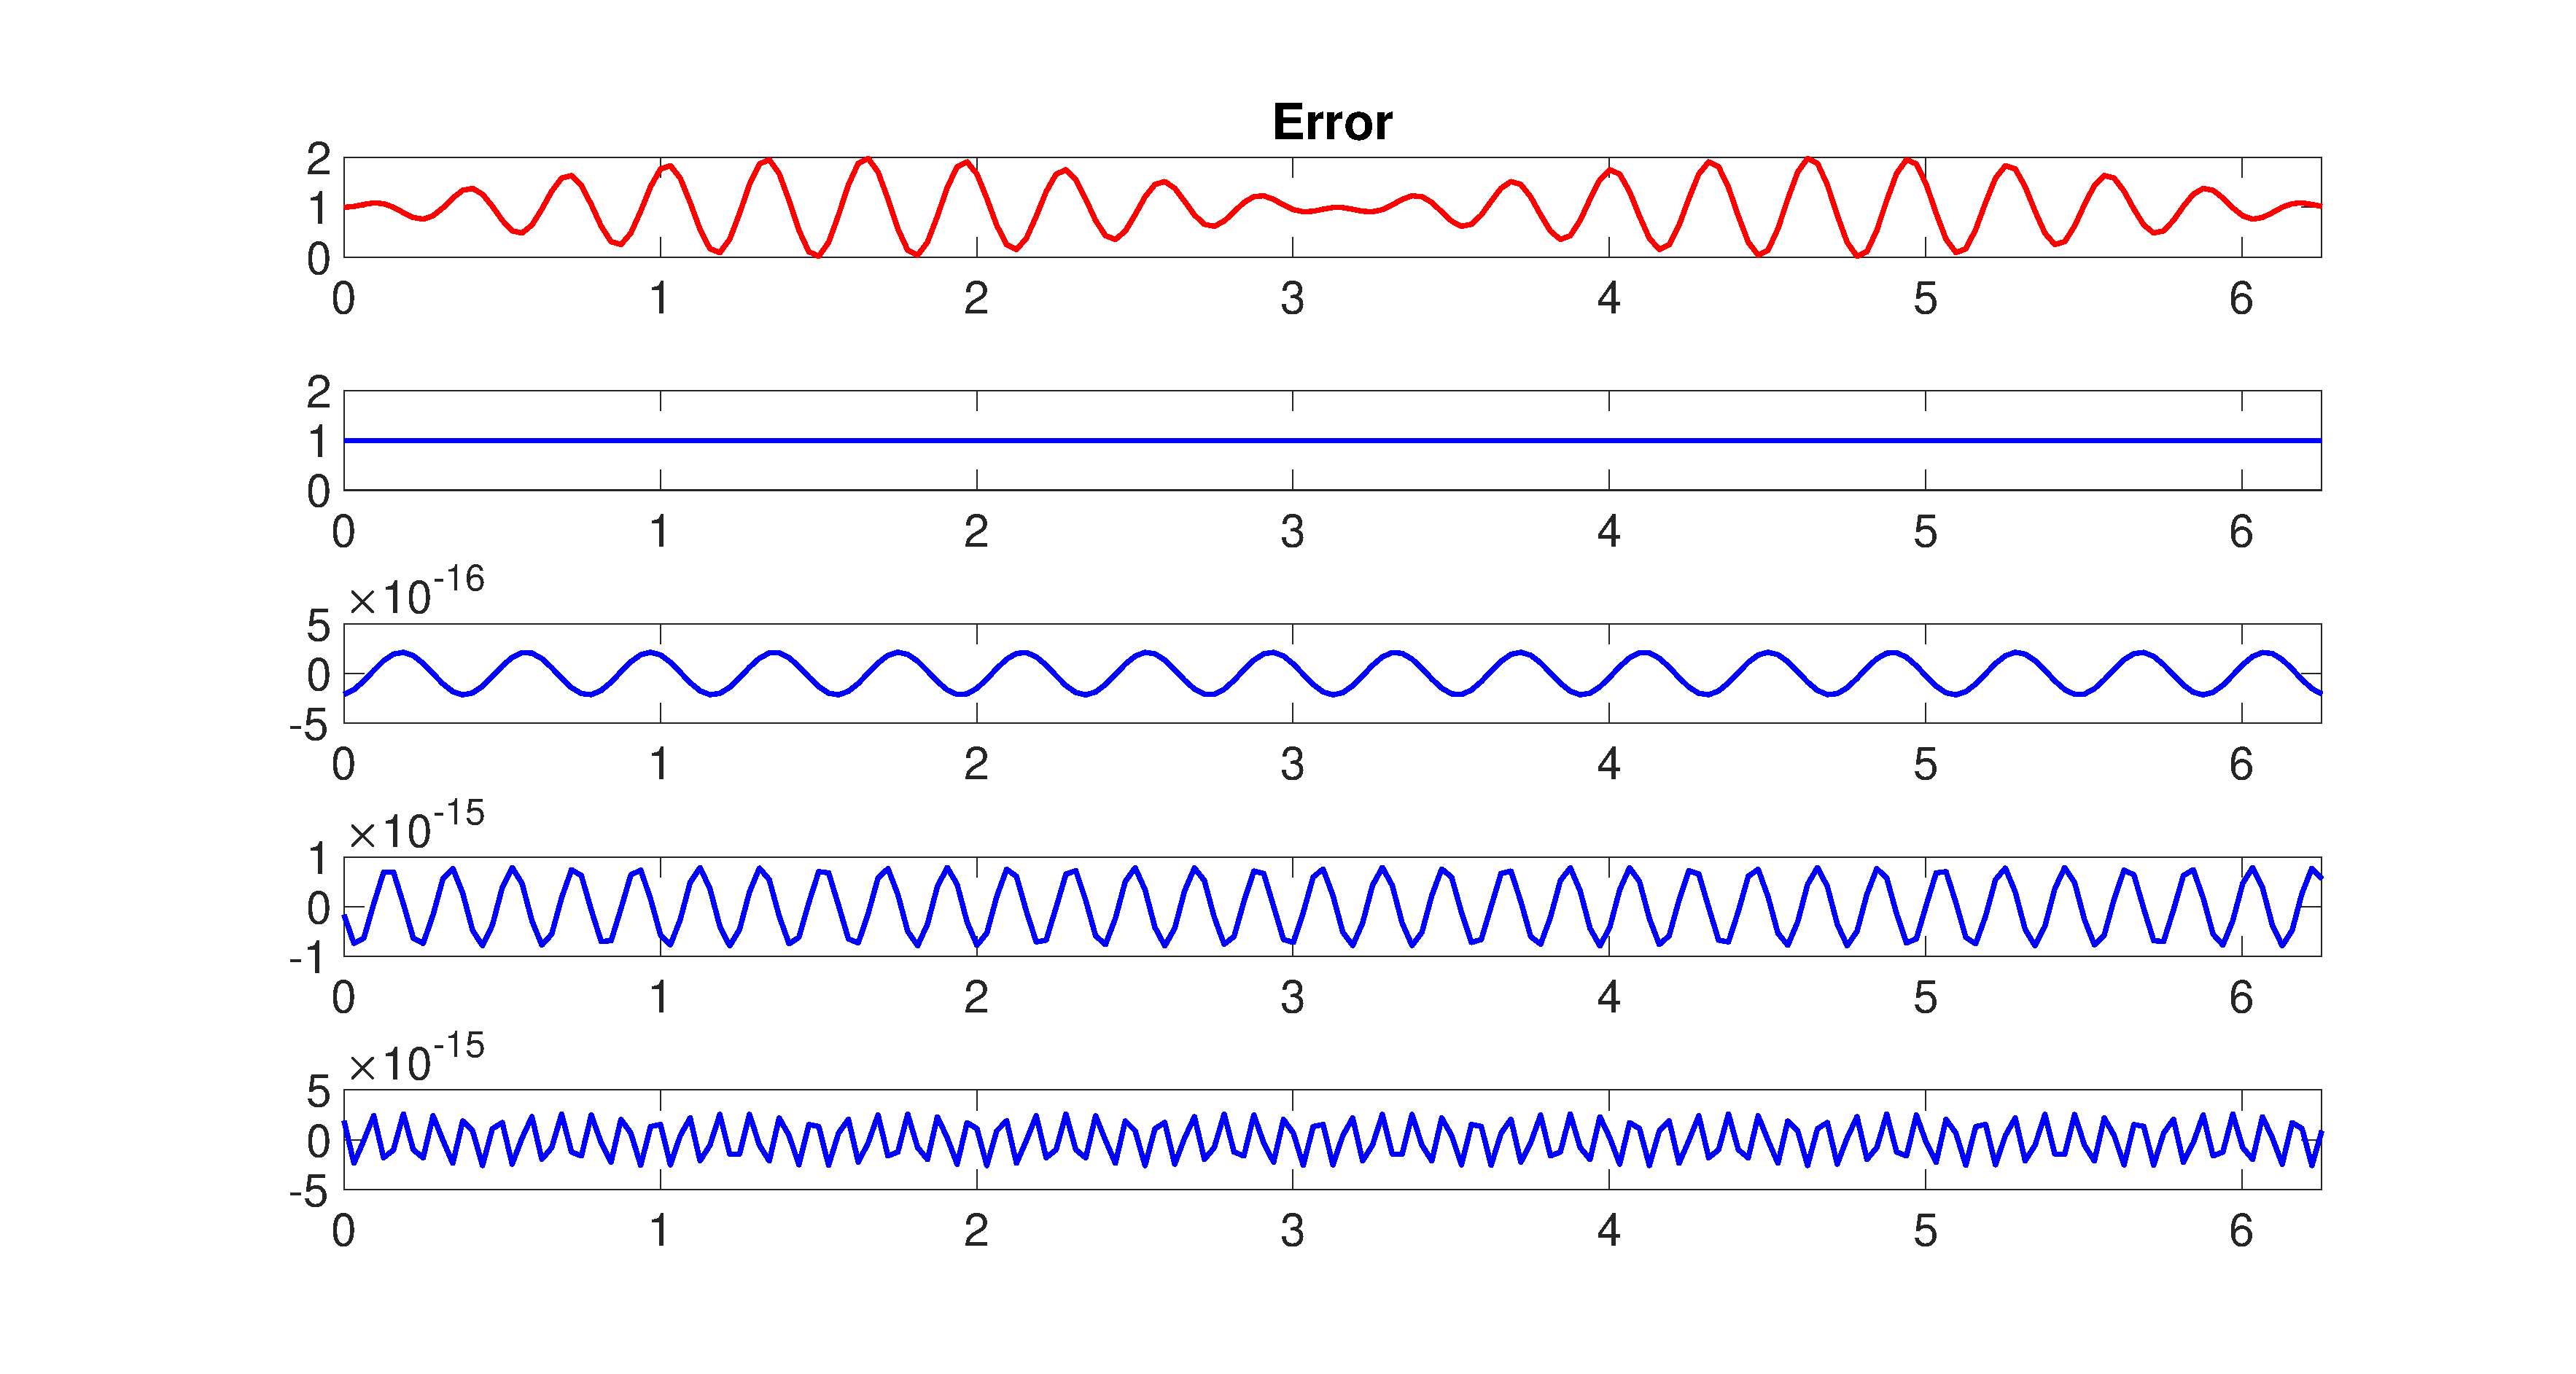
\includegraphics[width=0.8\textwidth]{img/errorfrequencydecomposition.eps}
		\label{abb_arc}
\end{figure}
 $\bullet$ Gau{\ss}-Seidel smooths $H^1$, \textbf{but not} $H_{\text{div}}$,  high frequencies of the error;\\
$\bullet$ The kernel $\text{Ker}(\text{div})=  \left\lbrace \btau \in H_{\text{div}}, \tdiv \btau =0   \right\rbrace $ is too large;\\
$\bullet$ Patch-smoother for divergence-free components of the error;
\end{frame}



%%%%%%%%%%%%%%%%%%%%%%%%%%%%%%%%%%%%%%%%%%
%%%%%%%%%%%                   SLIDE 6                %%%%%%%%%%%%%%%
%%%%%%%%%%%%%%%%%%%%%%%%%%%%%%%%%%%%%%%%%%

\begin{frame}
\titlecolor{Linear Multilevel: nested meshes and patches}
\footnotesize

\begin{figure}[htbp!]
	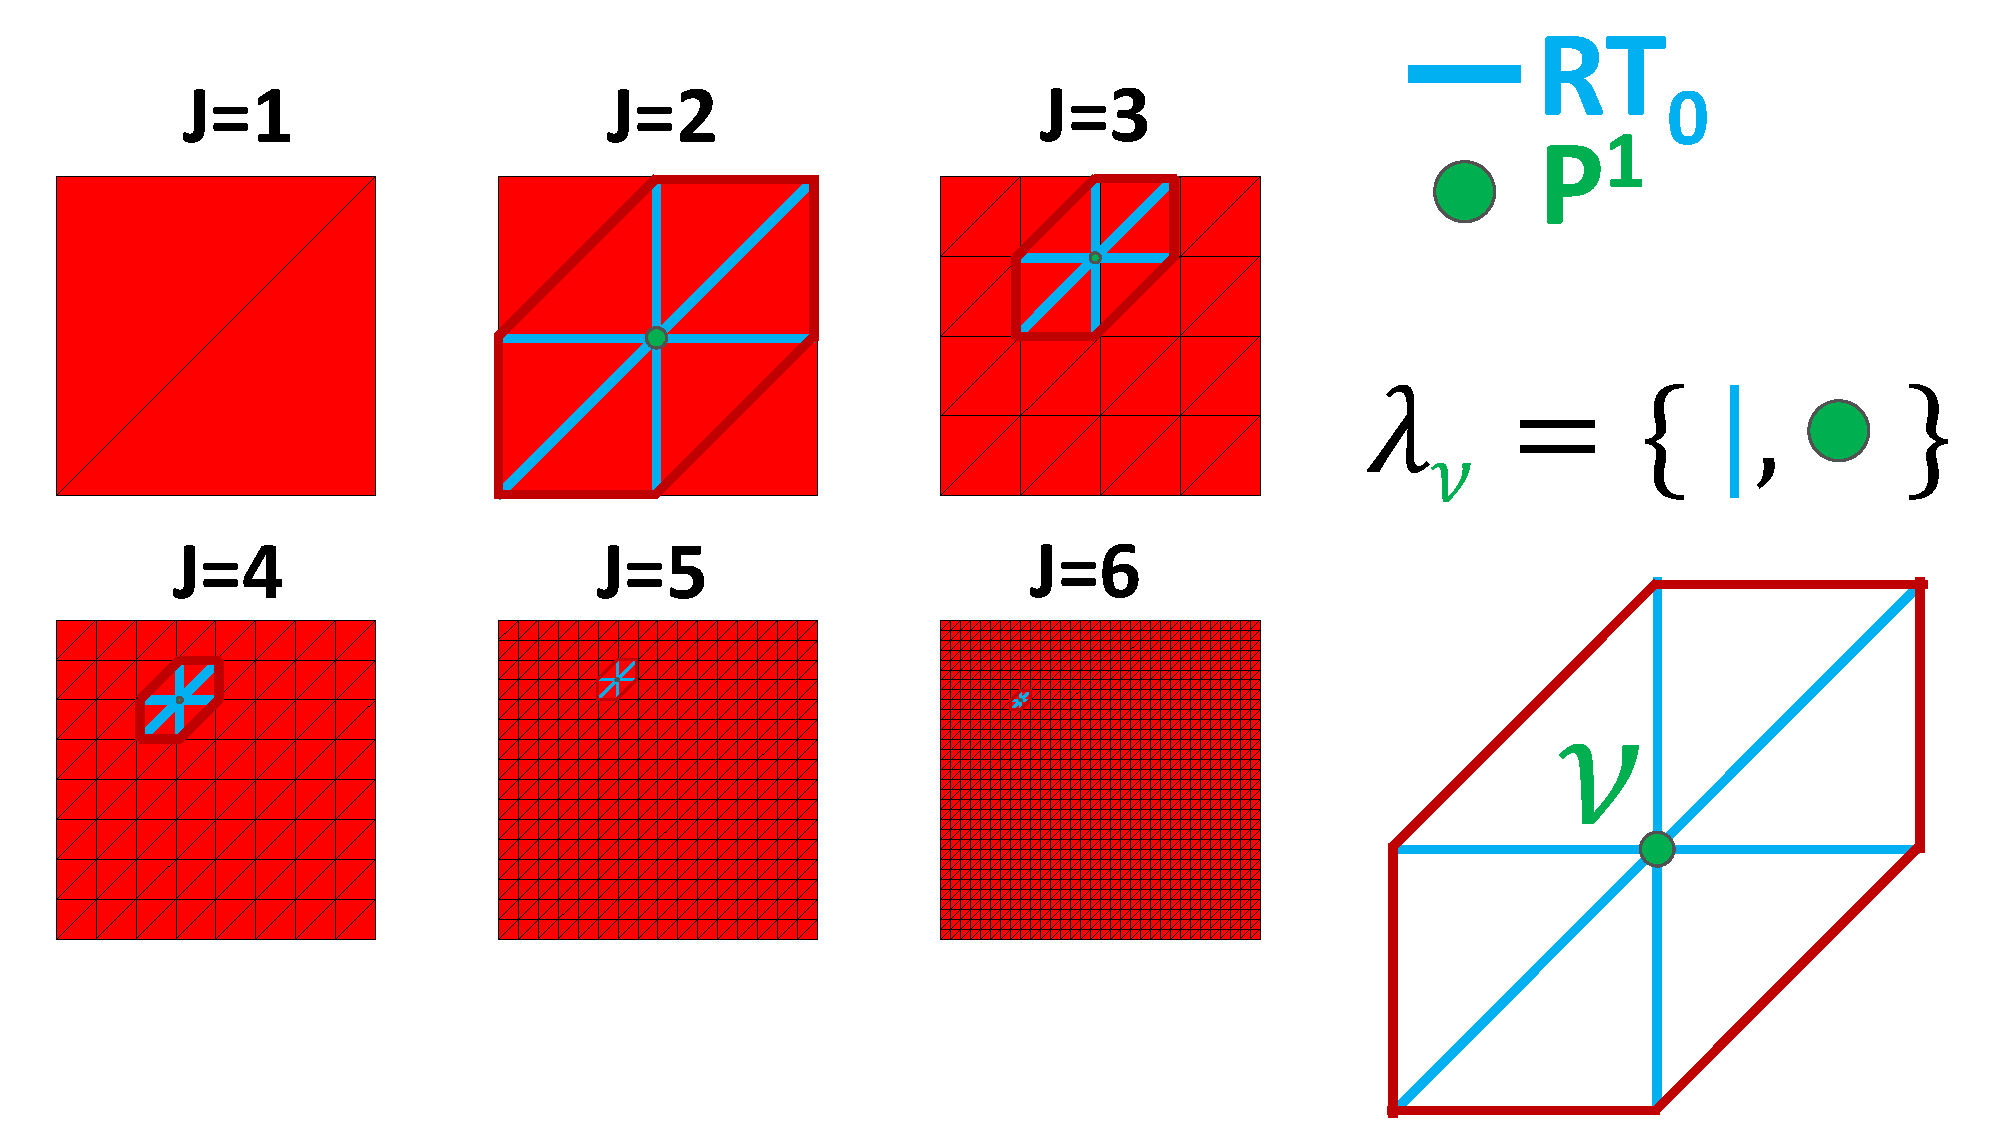
\includegraphics[width=0.8\textwidth]{img/refinementpatch.pdf}
		\label{abb_arc}
\end{figure}
$\bullet$ Minimization of the functional $\mathcal{J}(\bu,\bsigma)$ on $\text{span}(\lambda_{j,\nu})$\\
$\bullet$ Exploit $\nu$-patches to smooth the error in $H^1$ and $H_{\text{div}}$ simultaneously\\
${}$\\
\tiny{Ralf Hiptmair. Multigrid method for H(div) in three dimensions. Electron. Trans. Numer. Anal, 6(1):133-152, 1997.}${}$\\
${}$\\
\tiny{Douglas N Arnold, Richard S Falk, and Ragnar Winther. Multigrid in H(div) and H(curl). Numerische Mathe-
matik, 85(2):197-217, 2000.}
${}$\\
${}$\\
\tiny{
Gerhard Starke. Gauss-Newton multilevel methods for least-squares finite element computations of variably saturated subsurface flow. Computing, 64(4):323-338, 2000.}

\end{frame}












%%%%%%%%%%%%%%%%%%%%%%%%%%%%%%%%%%%%%%%%%%
%%%%%%%%%%%                   SLIDE 7                %%%%%%%%%%%%%%%
%%%%%%%%%%%%%%%%%%%%%%%%%%%%%%%%%%%%%%%%%%

\begin{frame}
\titlecolor{{Exact Monotone Multilevel}
Define:
\begin{itemize}
\item $\bbx_J^k=(\bu_J^k,\bsigma_J^k) \in K_J$  $k$-th iterate
\item $\bbx_{J,0}=\bbx_{J}^k$
\item $\bbx_{j,0}=\bbx_{j+1,N_{j+1}}$, for $j=J-1,...,1$
\end{itemize}
Compute a sequence of intermediate iterates $\bbx_{j,\nu} =\bbx_{j,\nu-1}+\bc_{j,\nu}$:
\begin{align*}
&\mathcal{J}%(\bbx_{j,\nu}+\bc_{j,\nu})
 \leq \mathcal{J}(\bbx_{j,\nu}+\by) 
\quad \forall \by \in K_{j,\nu}^{*}\qquad j=J,...,2, \quad \nu=1,...,N_j\\
& \mathcal{J}(\bbx_{2,N_2}+\bc_{1}) \leq \mathcal{J}(\bbx_{2,N_2}+\by) \quad \forall \by \in K_{1}^{*}  \qquad j=1
\end{align*}
with the \textbf{exact} local closed convex sets $K_{j,\nu}^*$ and $K_1^*$:
\begin{align*}
\begin{aligned}
&  K_{j,\nu}^{*}(\bbx_{j,\nu})=\left\lbrace
\by \in \text{span}\{\blambda_{j,\nu}\}: \quad \by +\bbx_{j,\nu} \in K_J
  \right\rbrace  \\
  &  K_{1}^{*}(\bbx_{2,N_2})=\left\lbrace
\by \in \text{span}\{\blambda_{1}\}: \quad \by +\bbx_{2,N_2} \in K_J
  \right\rbrace 
  \end{aligned}
\end{align*}
${}$\\
${}$\\
\tiny{
Ralf Kornhuber. Monotone multigrid methods for elliptic variational inequalities I. Numerische Mathematik, 69(2):167-184, 1994.}
${}$\\${}$\\
\tiny{
 Ralf Kornhuber and Rolf Krause. Adaptive multigrid methods for Signorini's problem in linear elasticity. Computing and Visualization in Science, 4(1):9-20, 2001.}
\end{frame}



%%%%%%%%%%%%%%%%%%%%%%%%%%%%%%%%%%%%%%%%%%
%%%%%%%%%%%                   SLIDE 8                %%%%%%%%%%%%%%%
%%%%%%%%%%%%%%%%%%%%%%%%%%%%%%%%%%%%%%%%%%

























\begin{frame}

\end{frame}
\begin{frame}

\end{frame}

\begin{frame}

\end{frame}



\begin{frame}
\frametitle{\textbf{Signorini problem: strong formulation}}
\begin{itemize}
\item Linear Elasticity:
\begin{align*}
\footnotesize
\begin{cases}
\text{div} \bsigma + \bff=0 & \Omega  \qquad \text{momentum balance equation}\\
\mathcal{A} \bsigma - \boldsymbol{\varepsilon}(\bu)=0 &\Omega \qquad \text{constitutive law}\\
\bu = \bu_d & \Gamma_D\qquad \text{Dirichlet BC}\\
\bsigma  \bn = \bt_n & \Gamma_N\qquad \text{Neumann BC}\\
\end{cases} \\
\end{align*}
\item Contact Constraints ($ \partial \Omega=\Gamma_C \cup  \Gamma_D \cup  \Gamma_N$, $\Gamma_i \cap  \Gamma_j =\emptyset$ for $i,j=D,N,C, i \neq j$):
\end{itemize}
\begin{align*}
\footnotesize
\begin{cases}
\bu \cdot \bn - g  \leq 0 \quad & \Gamma_C  \:\:  \text{impenetrability}\\
(\bsigma \bn) \cdot \bn \leq 0 \quad & \Gamma_C  \:\:  \text{direction of the surface pressure}\\
 \left(\bu \cdot \bn -g \right) \left( (\bsigma \bn) \cdot \bn \right) =0 &\Gamma_C  \:\:  \text{complementarity condition}
\end{cases}
\end{align*}
\begin{figure}[htbp!]
		\centering
	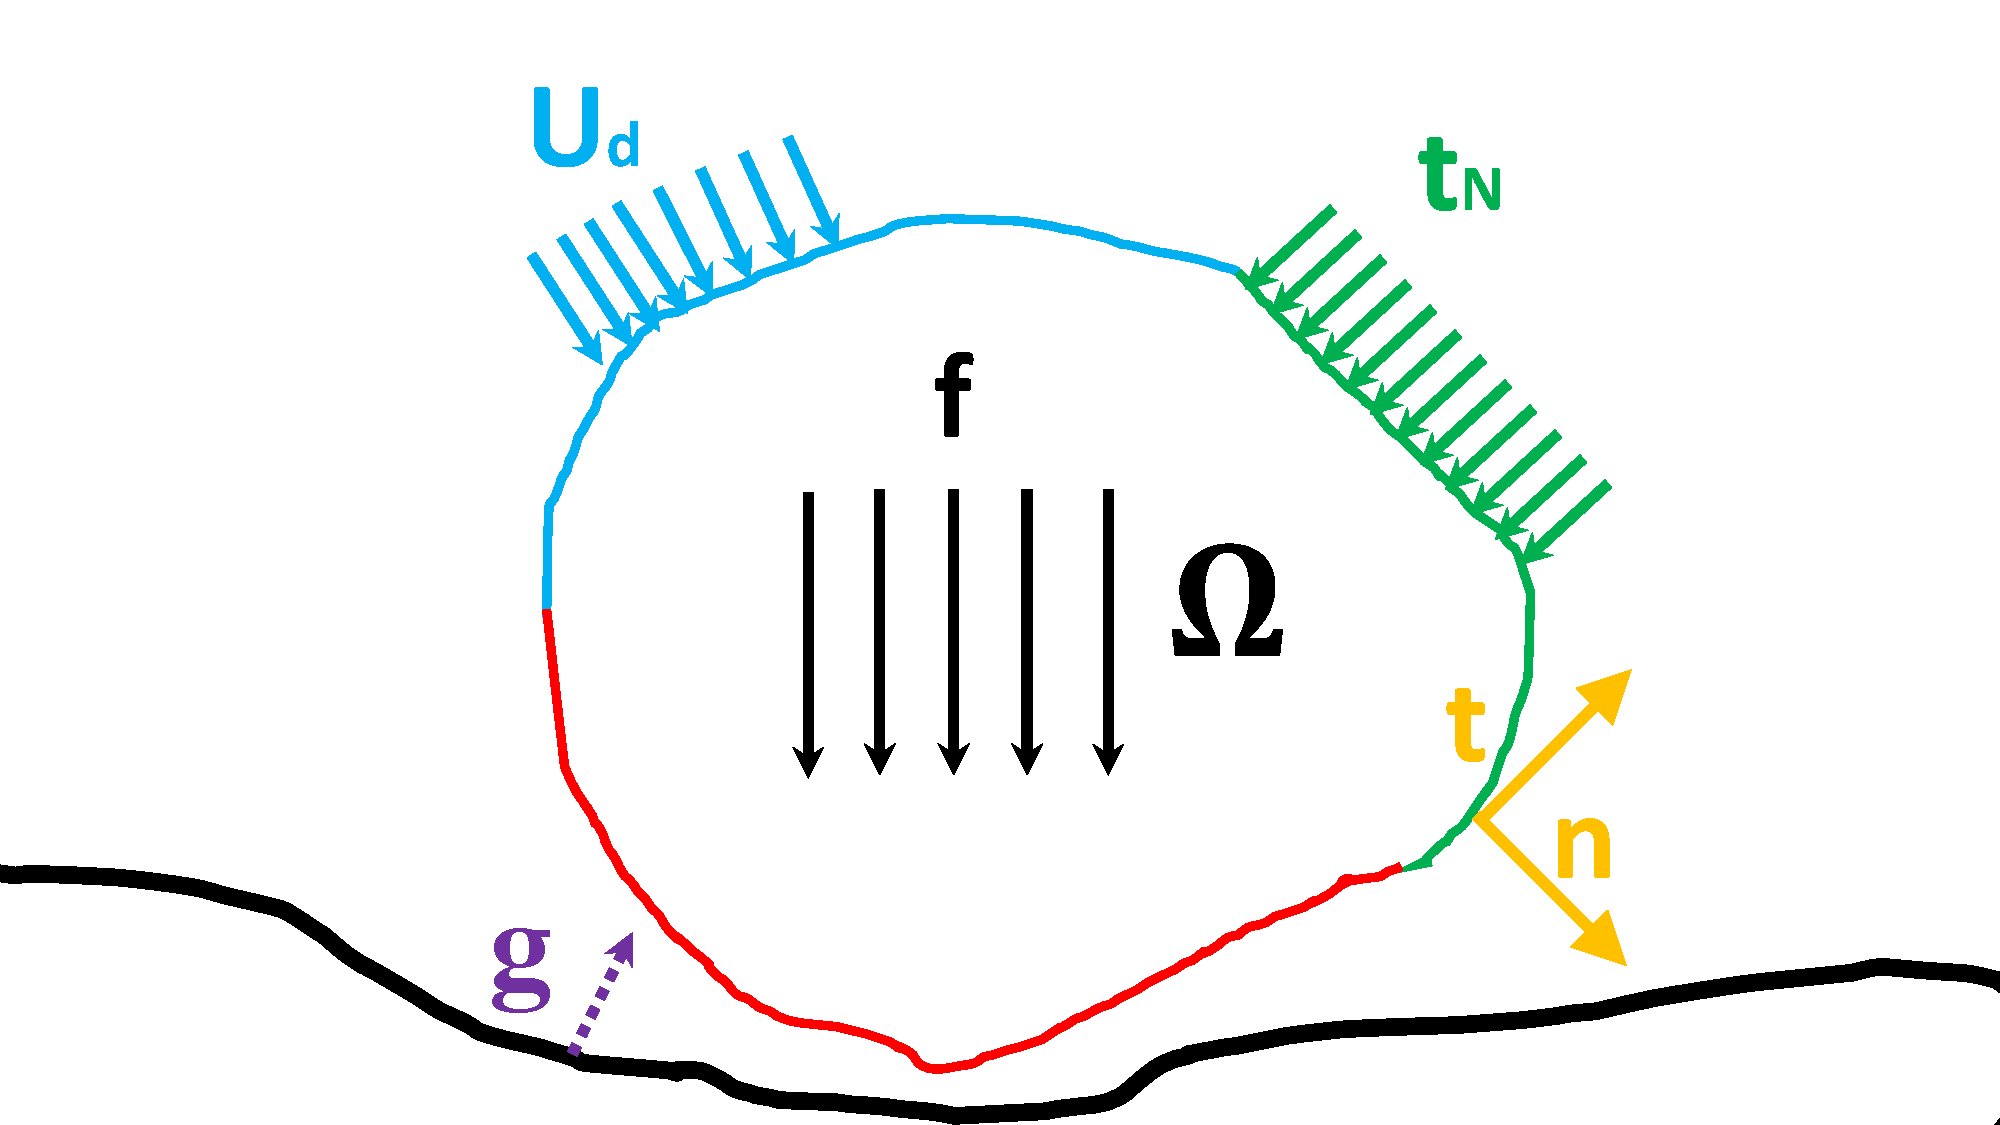
\includegraphics[width=0.3\textwidth]{img/contactproblem.pdf}
		\label{abb_arc}
\end{figure}
\footnotesize{Rolf Krause. A nonsmooth multiscale method for solving frictional two-body contact problems in 2d and 3d with multigrid efficiency. SIAM Journal on Scientific Computing, 31(2):1399–1423, 2009.}
\end{frame}






\begin{frame}
\frametitle{\textbf{Different formulations for Linear Elasticity}}
\begin{itemize}
\item \textbf{Displacement}:  
\begin{itemize}
\item Solve for displacements; stresses computed a posteriori
\item Unable to describe incompressible solids
\end{itemize}
\footnotesize
\begin{align*}
&\min \limits_{\bu\in H_{\Gamma_{d}}^1(\Omega)}\mathcal{J}(\bu)=\left(\bC \boldsymbol{\varepsilon}(\bu), \boldsymbol{\varepsilon}(\bu) \right)_{L^2 \left(\Omega \right)} - \left( \bff, \bu \right)_{L^2 \left(\Omega \right)}
\end{align*}
\item  \textbf{Hellinger-Reissner}: 
\begin{itemize}
\item Solve for displacements and stresses
\item Due to integration by parts: the stresses must be symmetric
\item Complex FEM spaces with large number of local dofs are required
\end{itemize}
\small
\begin{align*}
&\min \limits_{(\bu,\sigma) \in U_S}\mathcal{J}(\bu)=\frac{1}{2}\left(\mathcal{A} \bsigma, \bsigma \right)_{L^2 \left(\Omega \right)} + \left(\nabla \cdot \bsigma + \bff, \bu \right)_{L^2 \left(\Omega \right)} \\
\footnotesize
&U_S=\left[L^2(\Omega)\right]^d  \times \left[H_{\text{div}, \Gamma_N,S}^d(\Omega)\right]^d
\end{align*}
\item \textbf{Least-Square}: 
\begin{itemize}
\item Solve for displacements and stresses
\item Able to describe incompressible solids
\item No integration by parts: the stresses can be asymmetric
\item LS-functional as a posteriori error estimator
\end{itemize}
\footnotesize
\begin{align*}
& \min \limits_{(\bu,\bsigma) \in  U }\mathcal{J}(\bu,\bsigma)=C_{eq} ||\text{div} \bsigma+\bff||_{L^2(\Omega)^d}^2+C_{const}||\mathcal{A}\bsigma -\boldsymbol{\varepsilon}(\bu)||_{L^2(\Omega)^d}^2  +C_{asym}||\bsigma -\bsigma^T||_{L^2(\Omega)^d}^2  \\
& U=\left[H_{\Gamma_{d}}^1(\Omega) \right]^d \times \left[ H_{{\text{div},\Gamma_N}}(\Omega) \right]^d
\end{align*}
\end{itemize}
\footnotesize{Zhiqiang Cai and Gerhard Starke. Least-squares methods for linear elasticity. SIAM Journal on Numerical Analysis, 42(2):826–842, 2004} ${}$\\
${}$\\
\footnotesize{Brezzi, Franco, and Michel Fortin. Mixed and hybrid finite element methods. Vol. 15. Springer Science $\&$ Business Media, 2012.}
\end{frame}



\begin{frame}
\frametitle{\textbf{Least-Square Contact Linear Elasticity}}
\begin{itemize}
\item Non linear non-complementarity condition added to the functional
\item Solution searched in the convex set $K$
\item LS-functional non negative on $K$
\end{itemize}
\begin{align*}
\min \limits_{(\bu,\bsigma) \in  K}\mathcal{J}(\bu,\bsigma)=&C_{eq} ||\text{div} \bsigma+\bff||_{L^2(\Omega)^d}^2+C_{const}||\mathcal{A}\bsigma -\boldsymbol{\varepsilon}(\bu)||_{L^2(\Omega)^d}^2   +\\
&C_{asym}||\bsigma -\bsigma^T||_{L^2(\Omega)^d}^2 +C_{compl} \langle \bu \cdot \bn -g, (\bsigma \bn) \cdot \bn \rangle_{\Gamma_c}
\end{align*}
where:
\begin{align*}
 K=\{  \left(\bu,  \bsigma \right)  \in  \left[H_{\Gamma_{d}}^1(\Omega) \right]^d \times \left[ H_{\Gamma_{\text{div},\Gamma_N}}(\Omega) \right]^d    : \quad 
 \bu \cdot \bn - g  \leq 0, \quad  (\bsigma \bn) \cdot \bn \leq 0 \quad  \Gamma_C
 \}
\end{align*}
${}$\\
${}$\\
\footnotesize{Rolf Krause, Benjamin M\"{u}ller, and Gerhard Starke. An adaptive least-squares mixed finite element method for the signorini problem. Numerical Methods for Partial Differential Equations, 33(1):276–289, 2017.}

${}$\\
\footnotesize{Gerhard Starke, Alexander Schwarz, and Jo\"{o}rg Schr\"{o}der. Analysis of a modified first-order system least squares method for linear elasticity with improved momentum balance. SIAM Journal on Numerical Analy- sis, 49(3):1006–1022, 2011.}
\end{frame}


\begin{frame}
\frametitle{\textbf{BCs and LS a posteriori error estimator}}
\textbf{Least-Square Boundary conditions}:\\
\begin{itemize}
\item \textbf{ Strong/Essential boundary condition:} 
\begin{align*}
\bu=\bu^D \:\text{on}\:\Gamma_D, \quad  \bsigma \bn =\bt^N   \:\text{on}\:\Gamma_N
\end{align*}
\item \textbf{ Weak/Natural boundary condition:}
\begin{align*}
\mathcal{F}(\bu,\bv)=\mathcal{F}_{\text{0 bc}}(\bu,\bv)+C_D ||\bu-\bu^D ||_{H^{1/2(\Gamma_D)}}^2+C_N ||\bsigma \bn - \bt^N  ||_{H^{-1/2(\Gamma_N)}}^2
\end{align*}
Sum of different type of norms that are not equivalent.
\end{itemize}
\textbf{LS functional as an a posteriori error estimator}:\\
Let be $e$ the error and $|| \cdot||$ a proper norm. Then:
\begin{align*}
&C_1 ||\text{e}||  \overbrace{\leq}^{ \text{reliability} }  \mathcal{F} \overbrace{\leq}^{\text{efficiency}} C_2 ||\text{e}||  \quad \Rightarrow \quad
 ||\text{e}||   \to 0 \:\: \iff \:\: \mathcal{F} \to 0
\end{align*}
\footnotesize{Attia, Frank S., Zhiqiang Cai, and Gerhard Starke. "First-order system least squares for the Signorini contact problem in linear elasticity." SIAM Journal on Numerical Analysis 47.4 (2009): 3027-3043.}\\
${}$\\
\footnotesize{Starke, Gerhard. "Multilevel boundary functionals for least-squares mixed finite element methods." SIAM journal on numerical analysis 36.4 (1999): 1065-1077.}\\
${}$\\
\footnotesize{Bochev, Pavel B., and Max D. Gunzburger. Least-squares finite element methods. Vol. 166. Springer Science $\&$ Business Media, 2009.}
\end{frame}







\begin{frame}
\frametitle{\textbf{FEM Discretization}}
\begin{itemize}
\item $\bu_h \in H^1(\Omega)$: $P^1$ \textbf{Lagrange FEM}
\item $\bsigma_h \in H_{\text{div}}(\Omega)$: $\RT_0$ \textbf{Raviart-Thomas FEM}, \textbf{$H_{\text{div}}(\Omega)$-conforming}
\begin{itemize}
\item  \textbf{$\RT$-basis of order k}
\begin{align*}
RT_k(\Omega,T_h)& =\{q\in H_{\text{div}}(\Omega) : \: q|_k(K) \in RT_k(K), K\in T_h\}\\
RT_k(K) &=P_k(K)^d+  \bbx \tilde{P}_k(K)
\end{align*}
\item \textbf{DOFs}
\begin{enumerate}
\item Face-dofs:          $\qquad \quad \int_{\partial K} \bq \cdot \bn p_k d \sigma \qquad p_k \in R_k(\partial K)$
\item Momentum-dofs: $\int_{ K} \bq \cdot \bp_{k-1} d \bbx \qquad \bp_{k-1} \in P_{k-1}^d(\partial K)$
\end{enumerate}
\item \textbf{Local Dimension}
\begin{align*}
\dim RT_0(K)=\begin{cases}
3&d=2\\
4&d=3
\end{cases}
\end{align*}
\end{itemize}
\end{itemize}
${}$\\
${}$\\
${}$\\
\footnotesize{Marie E Rognes, Robert C Kirby, and Anders Logg. Efficient assembly of h(div) and h(curl) conforming finite elements. SIAM Journal on Scientific Computing, 31(6):4130–4151, 2009.}

\end{frame}

\begin{frame}
\Huge \center {Multilevel for Least Square Contact}
\end{frame}


\begin{frame}
\frametitle{\textbf{Novelty}}
\begin{itemize}
\item The LS-system coincides with the normal equations, $\bA^* \bA \bbx =\bA^* \bb$ \\
${}$
\item Ill-conditioned system: $K(A^* A) \leq K(A)^2$ \\
${}$
\item Need for fast solver: Multigrid MG \\
${}$
\item \textbf{Up to now}, no application of $H_{\text{div}}$ MG to LS Liner Elasticity, much less to LS contact problems.

\end{itemize}


\end{frame}


\begin{frame}
\frametitle{\textbf{Monotone Multigrid (MMG)}}
\begin{itemize}
\item MMG: energy reduction by subspace correction
\item  For a constrained problem: $U=U_1+...+U_n$ (solution space decomposition) and $K=K_1 +...+K_n$ (corresponding convex set decomposition), we search for:
\begin{align*}
u \in K : \mathcal{J}(u) \leq \mathcal{J}(v) \qquad \forall v \in K \subset U
\end{align*}
Given an initial iterate $w_0=u_{\nu}$, the following subproblems must be solved sequentially:
\begin{align*}
\mathcal{J}(w_i) =\min \limits_{v \in U_i, \:  w_{i-1}+v \in K } \mathcal{J}(w_{i-1}+v)   \qquad i=1,...,n
\end{align*}
\item The constraints are tackled locally. No need for global Lagrange Multipliers (but can be necessary at a local level)
\item We need MG for both $H^1$ and $H_{\text{div}}$
\end{itemize}
${}$\\
${}$\\
\footnotesize{Ralf Kornhuber. Monotone multigrid methods for elliptic variational inequalities i. Numerische Mathematik, 69(2):167–184, 1994.}
${}$\\${}$\\
\footnotesize{Ralf Kornhuber, Rolf Krause, O Sander, P Deuflhard, and S Ertel. A monotone multigrid solver for two body contact problems in biomechanics. Computing and Visualization in Science, 11(1):3–15, 2008.}


\end{frame}


\begin{frame}
\frametitle{\textbf{$H_{\text{div}}$ Multilevel}}
\textbf{MG prerequisite}: eigenfunctions associated to small eigenvalues can be well represented on coarse meshes.
\begin{align*}
\begin{cases}
\Lambda_{H^1}(\bu,\bv)=(\bu,\bv)+(\nabla \bu,\nabla \bv) \\
\lambda_{H^1}=1+\frac{|\nabla \bu|_1^2}{||\bu||_{L^2}^2}
\end{cases}
\qquad 
\begin{cases}
\Lambda_{H^{\text{div}}}(\bu,\bv)=(\bu,\bv)+(\text{div} \bu,\text{div} \bv)\\
\lambda_{H^{\text{div}}}=1+\frac{|\text{div} \bu|_1^2}{||\bu||_{L^2}^2}
\end{cases}
\end{align*}
\begin{itemize}
\item True in $H^1$: $\lambda_{H^1} \to \min \lambda_{H^1} \iff |\nabla \bu|_1 \to 0$
\item False in $H_{\text{div}}$: $\exists$ $\bu$, $\text{div} \bu = 0$ with $|\nabla \bu|_1 \gg 1$
\item Standard $H^1$ MG cannot be used in $H_{\text{div}}$. Usual smoothers are not able to dump error components on coarser meshes. Then choose between:
\begin{itemize}
\item Auxiliary Space Preconditioning
\item Arnold's smoother
\end{itemize}
\end{itemize}
${}$\\
${}$\\
\footnotesize{Ralf Hiptmair. Multigrid method for h (div) in three dimensions. Electron. Trans. Numer. Anal, 6(1):133–152, 1997.}${}$\\
${}$\\
\footnotesize{Ralf Hiptmair and Andrea Toselli. Overlapping and multilevel schwarz methods for vector valued elliptic prob- lems in three dimensions. In Parallel solution of partial differential equations, pages 181–208. Springer, 2000.}
\end{frame}

\begin{frame}
\frametitle{\textbf{Nodal Auxiliary Preconditioning}}
\begin{itemize}
\item Given $U$ solution space, let be: 
\begin{align*}
\bar{U}=U \times W_1 \times.. \times W_J \qquad \bar{u}=u + w_1 ...+w_J
\end{align*}
where $W_i=\Pi_i  \Phi_i $, with $ \Pi_j: W_j \to {U}$ is a transfer operator and $\Phi_i $ is a potential space.
\item The problem written in terms of the potential variable $\phi_i \in \Phi_i$ can be solved with standard MG.
\item Define Additive (A) and Multiplicative (M) Schwarz:
\begin{align*}
B_A=S^{-1}+\sum_{j=1}^J \Pi_j A_j^{-1} \Pi_j^* \qquad B_M=(\prod_{j=1}^J \Pi_j A_j^{-1}\Pi_j^* )S^{-1}
\end{align*}
\item Due to $\Pi_j$, it is difficult to deal with constraints in the spaces $W_j$.\\
Example: $\bar{u}=\bpsi + \bcurl p$ ($\bpsi  \in H^1$, $p \in H_{\bcurl}$)
\item Furthermore only $H_{\text{div}}$ is tackled. $H^1$ has to be considered separately.  
\end{itemize}

${}$\\
\footnotesize{Jinchao Xu. The auxiliary space method and optimal multigrid preconditioning techniques for unstructured grids. Computing, 56(3):215–235, 1996.}
${}$\\
${}$\\
\footnotesize{Ralf Hiptmair and Jinchao Xu. Nodal auxiliary space preconditioning in h (curl) and h (div) spaces. SIAM Journal on Numerical Analysis, 45(6):2483–2509, 2007.}
\end{frame}



\begin{frame}
\frametitle{\textbf{Special Case: Hiptmair's Smoother}}
Define $\bar{\bu}=\br +\bcurl \bphi$ and $\textbf{res}=\bff-\bA\br$.
\begin{align}
 \langle \bA\: (\br + \bcurl \bphi) , \btau \rangle = \langle \bff , \btau \rangle 
\quad & \rightarrow \quad \langle \bA \br, \btau \rangle + \langle\bA \bcurl \bphi , \btau \rangle = \langle \bff , \btau \rangle 
\end{align}
Then by choosing $\btau= \bcurl \bpsi $:
\begin{align}
\langle\bA \bcurl \bphi , \btau \rangle = \langle \bff - \bA \br, \btau \rangle \quad & \rightarrow \quad
\langle \bA\bcurl \bphi , \bcurl \bpsi \rangle  =\langle \textbf{res} ,  \bcurl \bpsi \rangle  \quad \forall \bpsi
\end{align}
\begin{itemize}
\item Choose $\br_0$
\item FOR k=1:N 
\begin{itemize}
\item Solve approximately for $ \langle \bA\: \br  , \btau \rangle =\langle \bff -\bA\: \br_k , \btau \rangle $
\item  Update $\br_{k+0.5}=\br_{k} + \br$ and define $ \textbf{res}_k= \bff-\bA\br_{k+0.5}$. 
\item Solve $\langle \bA\bcurl \bphi , \bcurl \bpsi \rangle  =\langle \textbf{res} ,  \bcurl \bpsi \rangle $
\item Update $\br_{k+1}=\br_{k+0.5}+\bcurl \bphi$
\end{itemize}
\end{itemize}
Problem: how to apply the boundary conditions on $\bphi$? If this is true (and I think it should be):
\begin{align*}
\bu \cdot \bn = \bh \quad \to \quad \bcurl \bphi \cdot \bn = \bh
\end{align*}
Since $\bphi \in \ND$, such a boundary condition is not local anymore and cannot be dealth with smoother that divide by the elements of the main diagonal (Jacobi, Gauss-Seidel...).
\end{frame}


\begin{frame}
\frametitle{\textbf{Arnold's Smoother}}
\begin{itemize}
\item Divergence-free functions are solenoidal: for their representation, at least a patch is needed.
\begin{figure}[htbp!]
		\centering
	\includegraphics[width=0.3\textwidth]{img/freedivergence.pdf}
		\label{abb_arc}
\end{figure}
\item Arnold's Smoother acts upon a whole patch, with a simultaneous subspace correction for $\bu$ and $\bsigma$. 
\footnotesize{
\begin{align*}
&\forall \nu=\text{node} \in T_h:
\qquad
1)
\begin{cases}
\min \limits_{\delta \bsigma_{\nu} \in \bSigma_h } \mathcal{F}(\bu_{\nu}^k ,\bsigma_{\nu}^k+ \delta \bsigma_{\nu} ) \quad \:\:\: \bsigma_{\nu}^{k+\frac{1}{2}}=\bsigma_{\nu}^k+\delta \bsigma_{\nu}\\
\min \limits_{\delta \bu_{\nu} \in \bU_h} \mathcal{F}(\bu_{\nu}^k+ \delta \bu_{\nu} ,\bsigma_{\nu}^{k+\frac{1}{2}} ) \quad \bu_{\nu}^{k+1}=\bu_{\nu}^k+\delta \bu_{\nu},
\end{cases}
\end{align*}
}
\item 
\normalsize
At least for the fine level,  the projection operators are not needed for the application of constraints.
\item No differentiation between $H^1$ and $H_{\text{div}}$.
\end{itemize}
 ${}$\\

 ${}$\\
\footnotesize{Douglas Arnold, Richard Falk, and Ragnar Winther. Preconditioning in h (div) and applications. Mathematics
of Computation of the American Mathematical Society, 66(219):957–984, 1997.}
${}$\\
${}$\\
\footnotesize{Douglas N Arnold, Richard S Falk, and Ragnar Winther. Multigrid in h (div) and h (curl). Numerische Mathe-
matik, 85(2):197–217, 2000.}
${}$\\
${}$\\
\footnotesize{
Gerhard Starke. Gauss–newton multilevel methods for least-squares finite element computations of variably saturated subsurface flow. Computing, 64(4):323–338, 2000.}


\end{frame}



\begin{frame}
\Huge \center {Numerical Experiments }
\end{frame}












\begin{frame}
\frametitle{\textbf{Asymmetric Weak Formulation for Linear Elasticity}}
The standard symmetric weak formulation for LS linear elasticity:
\begin{align*}
\small
 \begin{cases}
C_{eq}(\text{div} \bsigma , \text{div} \btau) + C_{const} (\mathcal{A} \bsigma,\mathcal{A} \btau) - C_{const}(\boldsymbol{\varepsilon}(\bu),\mathcal{A} \btau)=-C_{eq}(\bff , \text{div} \btau) & \forall \btau \in \left[ H_{\Gamma_N^0}^{\text{div}}(\Omega) \right]^d \\
- C_{const}(\boldsymbol{\varepsilon}(\bv),\mathcal{A} \bsigma)+
C_{const}(\boldsymbol{\varepsilon}(\bu),\boldsymbol{\varepsilon}(\bv))=0 & \forall \bv \in \left[H_{\Gamma_{d}^0}^1(\Omega) \right]^d\\
\bu = \bu^D & \Gamma_D\\
\bsigma  \bn = \bt^N & \Gamma_N\\
 \end{cases}
\end{align*}
can be replaced by an asymmetric formulation with improved momentum balance convergence:
\begin{align*}
\small
 \begin{cases}
C_{eq}(\text{div} \bsigma , \text{div} \btau) + C_{const} (\mathcal{A} \bsigma,\mathcal{A} \btau) - C_{const}(\boldsymbol{\varepsilon}(\bu),\mathcal{A} \btau)=-C_{eq}(\bff , \text{div} \btau) & \forall \btau \in \left[ H_{\Gamma_N^0}^{\text{div}}(\Omega) \right]^d \\
- C_{const}(\nabla \bv,\mathcal{A} \bsigma)+
C_{const}(\boldsymbol{\varepsilon}(\bu),\boldsymbol{\varepsilon}(\bv))=0 & \forall \bv \in \left[H_{\Gamma_{d}^0}^1(\Omega) \right]^d\\
\bu = \bu^D & \Gamma_D\\
\bsigma  \bn = \bt^N & \Gamma_N\\
 \end{cases}
\end{align*}
${}$\\
\footnotesize{Gerhard Starke, Alexander Schwarz, and Jo\"{o}rg Schr\"{o}der. Analysis of a modified first-order system least squares method for linear elasticity with improved momentum balance. SIAM Journal on Numerical Analy- sis, 49(3):1006–1022, 2011.}
\end{frame}













\begin{frame}
\frametitle{\textbf{Conclusion}}
\begin{itemize}
\item LS contact linear elasticity for good approximation of stresses and tackling of incompressible solids
\item Monotone MG with Arnold's smoother for a fast solver able to tackle the constraints locally. 
\end{itemize}
Future work:
\begin{itemize}
\item Understanding how to deal with the local constraints
\item Parallelization with patch smoothers: need for partition of unity
\item Two body problems and Mortar method: does exist a biorthogonal basis for $\RT$?
\item Implementation in 2D and in 3D 
\end{itemize}
\end{frame}


\begin{frame}
\center
\LARGE
Thank you for your attention!
\end{frame}


\begin{frame}
\end{frame}


\begin{frame}
\frametitle{\textbf{Problems and remarks}}
\textbf{HOW TO SOLVE THIS?}
I tried using ActiveSet with lagrange multipliers instead of the complementarity term. Comparing the results by Displacement Formulation on a square of 2 elements, it does not work.
\begin{align*}
\small
\min \limits_{(\bu,\bsigma) \in  K}\mathcal{J}(\bu,\bsigma)=&C_{eq} ||\text{div} \bsigma+\bff||_{L^2(\Omega)^d}^2+C_{const}||\mathcal{A}\bsigma -\boldsymbol{\varepsilon}(\bu)||_{L^2(\Omega)^d}^2   +\\
&C_{asym}||\bsigma -\bsigma^T||_{L^2(\Omega)^d}^2 +C_{compl} \langle \bu \cdot \bn -g, (\bsigma \bn) \cdot \bn \rangle_{\Gamma_c}
\end{align*}
Computing the discrete system:
\begin{align*}
\bA \bbx = \bb
\end{align*}
where:
\begin{align*}
 \bu \cdot \bn - g  \leq 0, \quad  (\bsigma \bn) \cdot \bn \leq 0
\end{align*}
do I have to satisfy these locally? \\
Node and edge normals/dofs positions are different.\\
On 1 edge, we have 2 displacement. On 1 node, we have 2 displacements.
\end{frame}

\begin{frame}
\frametitle{\textbf{Problems and remarks}}
Change reference coordiantes into local ones:
\begin{align*}
&2D: \qquad \bu = u_n \bn + u_t \bt \qquad \bsigma \bn = \sigma_n \bn + \sigma_t \bt \\
&3D: \qquad \bu = u_n \bn + u_{t,1} \bt_1 + u_{t,2} \bt_2 \qquad \bsigma \bn = \sigma_n \bn +\sigma_{t,1} \bt_1 + \sigma_{t,2} \bt_2
\end{align*}
Then we know that $\bbx= M_{nt} \bbx_{nt}$, so we can define $A_{nt}=A M_{nt} $ and solve:
\begin{align*}
A_{nt}  \bbx_{nt} =\bb \qquad \to \quad \bbx= M_{nt} \bbx_{nt}
\end{align*}
In this way I can decouple normal and tangent components of displacements and stresses and tackle directly the constraints.\\
${}$\\
In frictionless case, is it right to enforce $\sigma_t=0$, leaving $u_t$ free? To me it is, but I tried and it is not.Why?
\end{frame}


\begin{frame}
\frametitle{\textbf{Problems and remarks}}
\begin{itemize}
\item The computation of the pressure. We can compute the pressure as:
\begin{itemize}
\item $p=\bn^t \bsigma \bn$, where since we test again the normal, only the shape function related to this normal survives.
\item or we can define it as:
\begin{align*}
& p=\dfrac{1}{d} \left(\sum \limits_1^d \lambda_i \right) \qquad \left(\bsigma - \lambda_i  \textbf{I} \right) \bv =\textbf{0}\\
& \bsigma_e= \sum_{m \in T_e} \begin{bmatrix}
C_{1,m} \quad \bphi_{m}\\
C_{2,m} \quad \bphi_{m}\\
\end{bmatrix}, \qquad T_e \text{ element to which e belongs}
\end{align*}
where the stress, evaluated in the midpoint of the edge depends on all the shape functions  and coefficients of that element. \\
But, in principle, the other coefficients can be whatever. There is a discrepancy between the two way of computing it. In the continuum they should be the same.
\end{itemize} 
\end{itemize}
\end{frame}

\begin{frame}
\frametitle{\textbf{Problems and remarks}}
\textbf{Complementarity term:
}\begin{align*}
\langle \bu \cdot \bn -g, (\bsigma \bn) \cdot \bn \rangle_{\Gamma_c}
\end{align*}
\begin{itemize}
\item \textbf{Normal of the body itself}: Which normal do we consider here? The edge normal or a linear combination of the node normals? But then for the definition of the stress, we need also the stresses inside the element, not only the edge.
\item \textbf{Normal of the obstacle}: Also in this case, for the definition of the stress, we need also the stresses inside the element, not only the edge.
\end{itemize}
\end{frame}


\begin{frame}
\frametitle{\textbf{Problems and remarks}}
\begin{enumerate}
\item We have two different normals, for edges and displacements. Is this a 'contradiction'? If we consider the displacement in a middlepoint of an edge, here the normal is the one of the edge or is it the average of the two nodal-normal of the edge?
\item 
We have discontinuity of normals for both displacement and stresses. We cannot evaluate it pointwise, so it this also why we deal with it in the functional? 
\item How to solve the problem with the constraints? When you wrote the paper, what did you do?\\
\item The complementarity term is non negative ONLY if applied to the stress and displacement that satisfy the constraints. Otherwise it could be whatever, in principle. So am I destryoing the SPD structure of the matrix? Is it worth it? Other ways to deal with the complementarity condition?
\item  In the formulation we have the complementarity condition inserted in the functional, but there is no lagrange multiplier there
\item  Do I have to use multipliers only for the inequality constraints?
\item  Do I have to enforce it only for one (stress or displacement) or for both?
\item  Regarding the tangent stress =0 , do I have to enforce it with a lagrange multiplier?
\item  Regarding friction, how to proceed?
\end{enumerate}
\end{frame}


\begin{frame}
\frametitle{\textbf{Why the patch is necessary as smoother}}
I think that, in addition to the free-divergence functions, there is 'another' reason for which we need a patch-smoother. After a nodal Gauss-Seidel step:\\
\textbf{Displacement formulation}
\begin{itemize}
\item Unknown: only displacement
\item Gradient: automatically changed, but it is not needed in the formulation
\end{itemize}
\textbf{Mixed formulation:
}\begin{itemize}
\item Unknown: displacement and stress (gradient)
\item Since displacement and its gradient are uncoupled, when we change the first one, we do not change the second one, although it should. 
\item This can be seen by the fact that moving a node, also its edges are effected. We cannot modify the nodal value independently of the edge/dofes surrounding values.
\end{itemize}
\begin{figure}[htbp!]
			\includegraphics[width=0.65\textwidth]{img/whypatch.pdf}
\end{figure}
\end{frame}


\begin{frame}
\frametitle{\textbf{Local algorithm to solve friction}}
\begin{itemize}
\item A node is:
\begin{align*}
\begin{cases}
\text{constrained}  &\iff \: \:\text{is in contact}\\
\text{unconstrained} &\iff \:\: \text{is not in contact}
\end{cases}
\end{align*} 
\item An edge/face is:
\begin{align*}
\begin{cases}
\text{unconstrained}  &\iff \: \:\text{all its nodes are in contact}\\
\text{constrained} &\iff \:\: \text{at least one node is not in contact}
\end{cases}
\end{align*} 

\end{itemize}

\end{frame}



\begin{frame}
\frametitle{\textbf{Local algorithm to solve friction}}
Consider a node on $\Gamma_C$ and the corresponding patch. \\
\textbf{if N is not in contact}

\begin{itemize}
\item The stress dofs on $\Gamma_C$ are enforced equal to zero
\item Solve the system
\item If $\bu_N \cdot \bn \geq g$, constrain the node and move to the other case
\end{itemize}

\textbf{If N is in contact}
\begin{itemize}
\item All the stress dofs on $\Gamma_C$ that have at least one node free are enforced equal to zero
\item Solve the \textbf{sticky} node system: 
\begin{itemize}
\item  The displacement is enforced as $\bu = g \bn$
\item Solve the linear system
\item  If $|\bsigma_T| \leq \mathcal{F} p_n$, done. Otherwise go to the non-sticky node system
\end{itemize}
\item Solve the \textbf{non-sticky} node system: 
\begin{itemize}
\item  With lagrange multipliers, add to the linear system the constraints:  $\bu = g \bn$, $\bsigma_T =- \mathcal{F} p_n \dfrac{\bu_t}{||\bu_t||}$
\item Solve the non-linear system with fixed-point iteration. 
\end{itemize}
\end{itemize}

The computations are simplified if written in terms of corrections and if the initial guess on the contact boundary is zero.\\
In such a case, it is not necessary to enforce to zero the stress of edges/faces that are not in contact. This means that we can reduce the dimension of the system to solve to: $\text{dim}\: (1 + N_{\bsigma,int} + N_{\bsigma,\Gamma_C})$
\end{frame}

\begin{frame}
\frametitle{\textbf{Local algorithm to solve friction}}
\begin{itemize}
\item In Arnold's smoother, only $H_{\text{div}}$ is considered.
\item This means that only internal dofs of a patch can be considered
\item In case of a FOSLS formulation, both primal and dual variables are present
\item Solving with GS for only the local internal dofs works for the linear case
\item In general the algebraic structure of internal dofs does not represent a local subproblem: the local boundary is both Dirichlet and Neumann $\to$ wrong!
\item We have to solve local physical problems. Given a patch, the external nodes are dirichlet bc, the other are free. 
\item The local problem cannot be extracted from the original matrix due to stress dofs on the boundary!
\item We have to build the global matrix and local matrices for each path
\end{itemize}
\end{frame}




\begin{frame}
\frametitle{\textbf{Necessary Symmetry of the Stress Tensor}}
\begin{itemize}
\item $C_{eq}=1000$, $C_{asym}=10$: more (and proper) bending $\to$  captured
\item $C_{eq}=1$, $C_{asym}=0$: less (and wrong) bending $\to$  captured
\end{itemize}
\begin{figure}[htbp!]
		\centering
	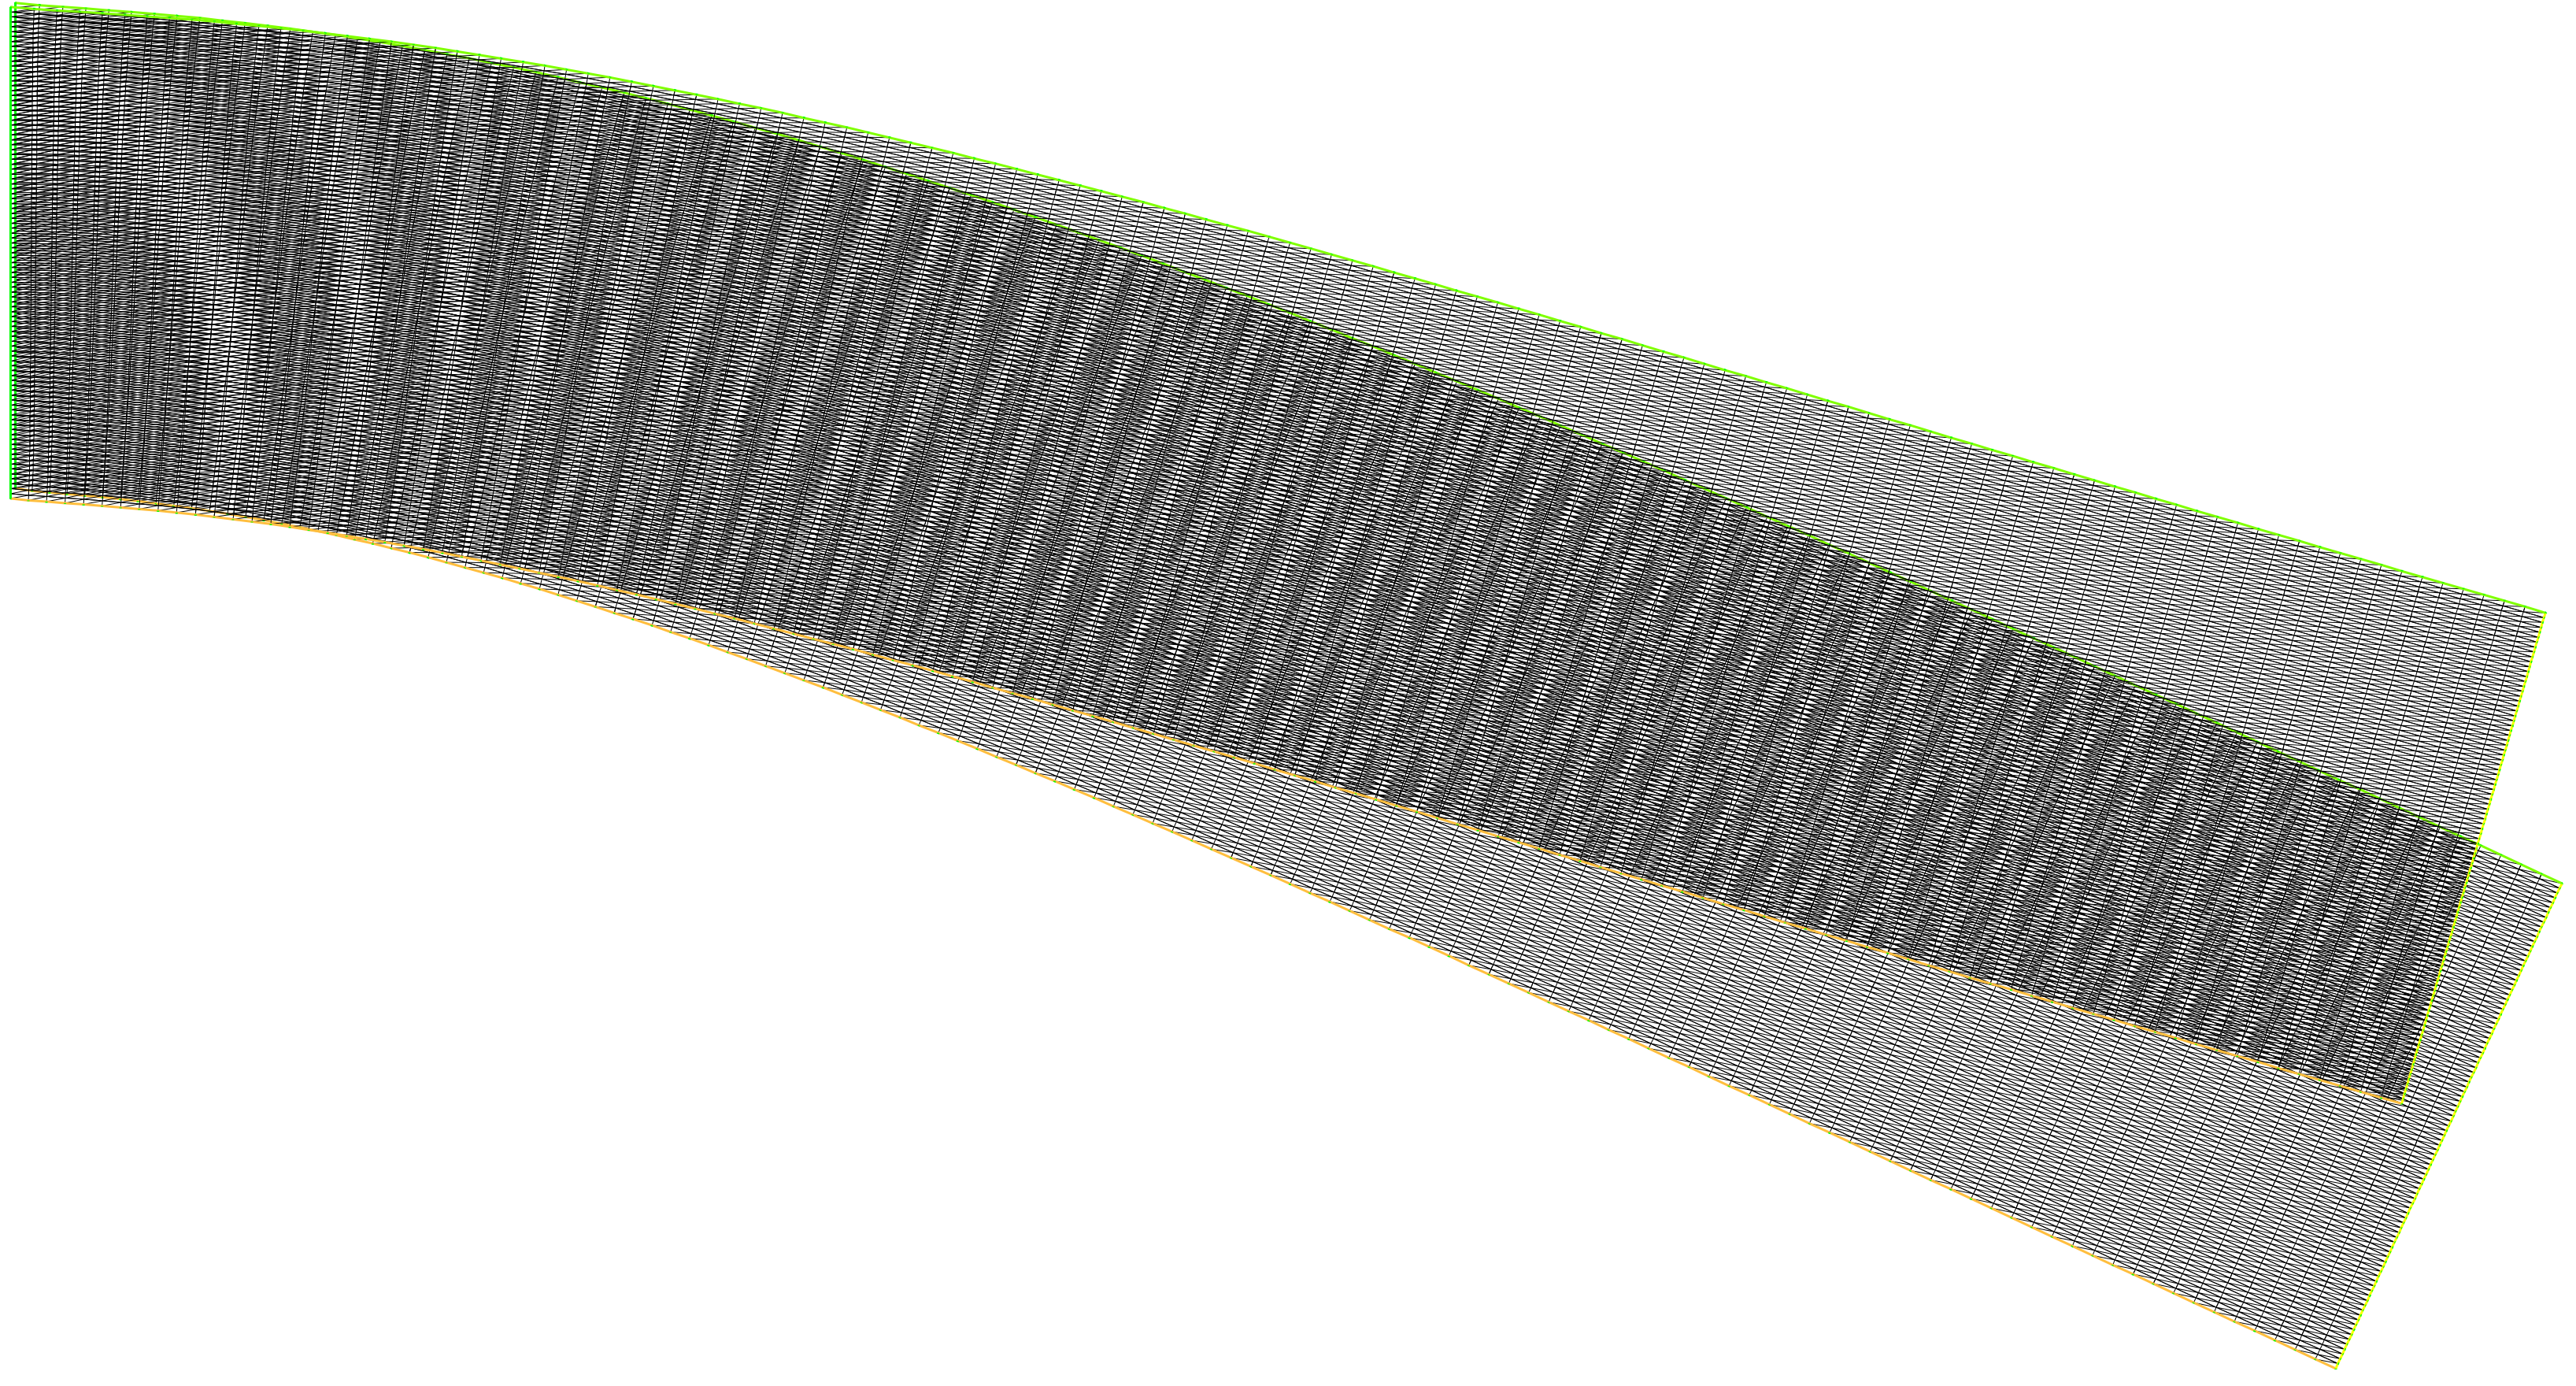
\includegraphics[scale=0.05]{img/nonbendingbeam}
\end{figure}
Symmetry of the stress tensor is necessary, but $C_{asym} \gg 1$ destroys Multigrid convergence.
\end{frame}

\end{document}  